%%%%%%%%%%%%%%%%%%%%%%%%%%%%%%%%%%%%%%%%%
% University Assignment Title Page
% LaTeX Template
% Version 1.0 (27/12/12)
%
% This template has been downloaded from:
% http://www.LaTeXTemplates.com
%
% Original author:
% WikiBooks (http://en.wikibooks.org/wiki/LaTeX/Title_Creation)
%
% License:
% CC BY-NC-SA 3.0 (http://creativecommons.org/licenses/by-nc-sa/3.0/)
%
% Instructions for using this template:
% This title page is capable of being compiled as is. This is not useful for
% including it in another document. To do this, you have two options:
%
% 1) Copy/paste everything between \begin{document} and \end{document}
% starting at \begin{titlepage} and paste this into another LaTeX file where you
% want your title page.
% OR
% 2) Remove everything outside the \begin{titlepage} and \end{titlepage} and
% move this file to the same directory as the LaTeX file you wish to add it to.
% Then add \input{./title_page_1.tex} to your LaTeX file where you want your
% title page.
%
%%%%%%%%%%%%%%%%%%%%%%%%%%%%%%%%%%%%%%%%%
%\title{Title page with logo}
%----------------------------------------------------------------------------------------
%	PACKAGES AND OTHER DOCUMENT CONFIGURATIONS
%----------------------------------------------------------------------------------------

\documentclass[12pt]{article}
\usepackage[toc,page]{appendix}
\usepackage[spanish]{babel}
\usepackage[utf8x]{inputenc}
\usepackage{pgfplots}
\usepackage{mathtools}
\usepackage{amsmath}
\usepackage{graphicx}
\usepackage{fancyhdr}
\usepackage[colorinlistoftodos]{todonotes}
\usepackage{changepage}
\usepackage[font=scriptsize]{caption}
\usepackage[a4paper,bindingoffset=0.2in,left=1in,right=1in,top=1in,bottom=0.5in,footskip=.25in]{geometry}
\usepackage[hidelinks]{hyperref}
\usepackage{eurosym}
\usepackage{MathUnicode}
\usepackage{amssymb}
\usepackage{amsthm}
\usepackage{pdfsync}
\usepackage{xspace,hyperref}
\usepackage{changepage}
\usepackage{float}
\usepackage{caption}
\usepackage{titlesec}
\usepackage{listings}
\usepackage{color} %red, green, blue, yellow, cyan, magenta, black, white
\usepackage{cleveref}

\definecolor{mygreen}{RGB}{28,172,0} % color values Red, Green, Blue
\definecolor{mylilas}{RGB}{170,55,241}
%\usepackage[numbered,framed]{matlab-prettifier}
\newcommand{\sectionbreak}{\clearpage}


\setlength{\arrayrulewidth}{1mm}
\setlength{\tabcolsep}{18pt}
\renewcommand{\arraystretch}{1.5}


\renewcommand{\labelitemii}{$\circ$}
\pagestyle{fancy}
\lhead{\textbf{Teoría del caos y fractales}}
%\chead{\leftmark}
\rhead{\leftmark}
%\rhead{\includegraphics[width=2.8cm]{img/logo_memo}}
%\rhead{\textbf{CyC}}

\newtheorem{theorem}{Teorema}[section]
\newtheorem{lemma}{Lema}[section]
\newtheorem{proposition}{Proposición}[section]
\theoremstyle{definition}
\newtheorem{definition}{Definición}[section]
\newtheorem{example}{Ejemplo}[section]

\renewcommand{\headrulewidth}{0.5pt}



\begin{document}

\begin{titlepage}

\newcommand{\HRule}{\rule{\linewidth}{0.5mm}} % Defines a new command for the horizontal lines, change thickness here

\center % Center everything on the page

%----------------------------------------------------------------------------------------
%	HEADING SECTIONS
%----------------------------------------------------------------------------------------

\textsc{\LARGE Universidad Autónoma de Madrid}\\[1.5cm] % Name of your university/college
\textsc{\Large Complejidad y Computación}\\[0.5cm] % Major heading such as course name


%----------------------------------------------------------------------------------------
%	TITLE SECTION
%----------------------------------------------------------------------------------------

\HRule \\[0.4cm]
{ \huge \bfseries Teoría del Caos y fractales}\\[0.4cm] % Title of your document
\HRule \\[1cm]


%----------------------------------------------------------------------------------------
%	AUTHOR SECTION
%----------------------------------------------------------------------------------------


% If you don't want a supervisor, uncomment the two lines below and remove the section above
\Large \emph{Autoress:}\\
Alejandro \textsc{Villegas}\\ % Your name
Elena \textsc{Gutiérrez}\\ % Your name
Miguel Ángel \textsc{González-gallego} \\
Pedro \textsc{Valero}\\[1cm] % Your name

%----------------------------------------------------------------------------------------
%	LOGO SECTION
%----------------------------------------------------------------------------------------

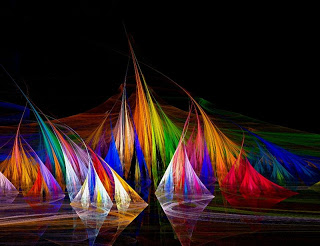
\includegraphics{img/Logo.jpg}\\ % Include a department/university logo - this will require the graphicx package

%----------------------------------------------------------------------------------------
%	DATE SECTION
%----------------------------------------------------------------------------------------

{\large \today}\\[1cm] % Date, change the \today to a set date if you want to be precise


%----------------------------------------------------------------------------------------

\vfill % Fill the rest of the page with whitespace

\end{titlepage}
\tableofcontents
\newpage

\section{Introducción}
Antes de comenzar a indagar en los fundamentos de la Teoría del Caos o en los fractales, debemos aclarar una serie de conceptos que aparecerán a lo largo de estos apuntes.

\begin{definition}[Sistema dinámico]\label{def:sistemaDinamico}
Un sistema dinámico es un sistema que consiste en un conjunto de estados, junto con una regla que determina el estado \emph{actual} en términos de los estados \emph{anteriores}.
\end{definition}

Los sistemas físicos en situación no estacionaria (es decir, los que varían con el tiempo) son ejemplos de sistemas dinámicos. También existen modelos económicos, matemáticos y de otros tipos que son sistemas abstractos y a la vez, son sistemas dinámicos.

Según las variables que intervienen en el sistema sean \textbf{discretas} (sólo tomen una serie de valores posibles) o \textbf{continuas} (pueden tomar cualquier valor dentro de un intervalo), así lo será el sistema.

Cuando definamos un sistema dinámico, exigiremos que la regla que lo rige sea determinista, es decir, una regla que nos permite conocer \emph{teóricamente} la evolución del sistema con total precisión. En particular, diremos que un sistema es \textbf{determinista} si es posible determinar su estado actual (p.e. la población de una cierta especie) \emph{solamente} a partir de los estados anteriores.

Es importante destacar el hecho de que los sistemas han de ser deterministas pues, de lo contrario, estaríamos hablando de procesos aleatorios, y por tanto, impredecibles. La \emph{idea clave} del concepto del Caos es que comprendemos el fenómeno y sabemos modelizarlo ``a la perfección'' pero el resultado futuro varía enormemente a partir de un pequeño cambio en los valores tomados del mundo real.


\begin{definition}[Teoría del Caos]
La teoría del Caos es la rama de las Matemáticas que estudia el comportamiento de sistemas dinámicos \emph{deterministas} muy sensibles a los datos iniciales.
\end{definition}
Surge al tratar de estudiar sistemas dinámicos no lineales, es decir, aquellos modelados por ecuaciones diferenciales o en diferencias, no lineales, los cuales presentan una dependencia extremendamente sensible a las condiciones iniciales. El efecto que observamos es que, en este tipo de sistemas, se puede comenzar con unas ciertas configuraciones iniciales muy cercanas pero estas comienzan a apartarse rápidamente mientras permanecen en una región acotada. Como el lector puede adivinar, el problema de estos sistemas caóticos es que es imposible predecir el comportamiento a largo plazo.
\begin{example}\label{example:Julia}
A modo de ejemplo podemos suponer un fenómeno que venga modelizado por la ecuación:
\[z_{n+1} = f(z_n) \text{ siendo } f(x) = x^2+1\]

Puesto que conocemos la ecuación que modela el fenómeno, queda claro que nos encontramos ante un sistema dinámico determinista, pues para todo valor de $n$ podemos calcular $z_{n+1}$.

Para un $n=11$, que no parece ser algo demasiado grande, siendo $z$ un número complejo, supongamos que cometemos un error muy pequeño, de la forma: $ε=10^{-5}+10^{-5}i$ al medir $z_0$.

En estas condiciones, la diferencia entre el valor obtenido y el original es
\[f^{11}(ε)=1.4 \cdot 10^{181} + 1.13\cdot 10^{174}i\]

Este ejemplo será estudiado con más detalle al hablar de los conjuntos de Mandelbrot.
\end{example}

También es fundamental aclarar, aunque algunos lectores pueden tener ya una idea intuitiva, qué es un \emph{fractal}.

\begin{definition}[Fractal]\label{def:fractal}
Un fractal es un objeto geométrico cuya estructura básica, fragmentada o irregular, se repite a diferentes escalas.
\end{definition}

Para poder comprender el concepto de fractal más allá de su definición veámos un ejemplo muy artificial pero muy ilustrativo.

\begin{example}
La idea básica de un fractal es que si nos fijamos en una pequeña parte de su estructura, observamos una repetición de la estructura global del objeto.

\begin{verbatim}
      A
     A A
    A   A
   A A A A
  A       A
 A         A
\end{verbatim}

Este dibujo tal cual se muestra \emph{no es un fractal} de verdad. Si cada símbolo $A$ que se muestra en el dibujo tuviese exactamente la misma forma que la letra representada con todas las $A$'s, entonces tendríamos realmente un fractal.
\end{example}

\section{Sistemas discretos}
\begin{definition}[Sistemas discretos]
Los sistemas dinámicos discretos son aquellos que en los que el tiempo se mide en pequeños lapsos.

Un reloj digital sería un sistema dinámico discreto mientras que un reloj analógico sería un sistema dinámico continuo.
\end{definition}

Para \emph{modelizar} los sistemas dinámicos discretos empleamos las ecuaciones en diferencias.

\subsection{Ecuaciones en diferencias.}

\begin{definition}[Ecuación en diferencias]
Una ecuación en diferencias es una expresión del tipo:
\[G(n,f(n),f(n+1),...,f(n+k))=0, \ \forall n \in \mathbb{Z}\]
donde $f$ es una función definida en $\mathbb{Z}$.
\end{definition}

\begin{example}
La ecuación en diferencias de primer orden:
\[X_{t+1} = F(X_t)\]
constituye un ejemplo de sistema dinámico determinista, siendo $F(x)$ una función conocida.
\end{example}

% Todo lo que viene a continuación viene de http://ltcconline.net/greenl/courses/204/firstOrder/differenceEquations.htm

A simple vista puede parecer que el ejemplo mencionado no es una ecuación en diferencias, puesto que no se aprecia ninguna derivada en la ecuación. No obstante, podemos escribir:
\[X'(t)=g(X(t)) \implies \lim_{h\to 0} \frac{X(t+h)-X(t)}{h}=g(X(t))\]

Puesto que los valores posibles de $t$ y $h$ son enteros, lo más pequeño que puede ser $h$ sin llegar a ser $0$ es $h=1$ con lo que tenemos:
\[g(X(t))=X'(t)=X(t+h)-X(t)=ΔX(t) \implies X(t+h) = X(t) +ΔX(t) \implies \atop F(X(t)) = X(t) + ΔX(t)\]

Por tanto, encontrar la función $X(t)$ que resuelve el sistema planteado en el ejemplo es equivalente a resolver la ecuación:
\[X(t+1)=X(t)+ΔX(t)\]
que, claramente, es una ecuación en diferencias.

\subsection{Ecuación logística}
\begin{definition}[Ecuación logística]
La función logística, curva logística o curva en forma de S es una función matemática que aparece en diversos modelos de crecimiento de poblaciones, propagación de enfermedades epidémicas y difusión en redes sociales.

Dicha función constituye un refinamiento del modelo exponencial para el crecimiento de una magnitud.
El estudio inicial de crecimiento es aproximadamente exponencial; al cabo de un tiempo, aparece la competencia entre algunos miembros de P por algún recurso crítico K (``cuello de botella'') y la tasa de crecimiento disminuye; finalmente, en la madurez, el crecimiento se detiene.
\end{definition}

La función logística simple se define mediante la fórmula
\[P(t) = \frac{1}{1+e^{-t}}\]
que da lugar a la gráfica \ref{fig:EcLogistica}.

\begin{figure}[hbtp]
\centering
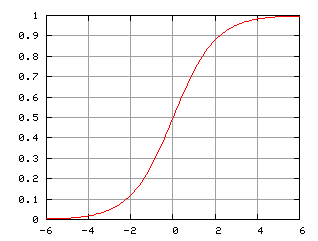
\includegraphics[width = 0.6\textwidth]{img/EcuacionLogistica.png}
\caption{Gráfica de $P(t) = \frac{1}{1+e^{-t}}$}
\label{fig:EcLogistica}
\end{figure}


El crecimiento logístico está relacionado con el crecimiento exponencial, de hecho para pequeños valores de la magnitud que presenta crecimiento logístico, el crecimiento logístico se asemeja mucho al crecimiento exponencial. Sin embargo, a partir de un cierto punto el crecimiento se ralentiza, eso hace que la curva pueda representar adecuadamente la propagación de rumores, la extensión de una innovación tecnológica o una epidemia: al principio estas se propagan rápidamente, cada ``infectado'' o ``afectado'' por la innovación es susceptible de traspasar el ``contagio'' a otro individuo que tenga contacto con él, pero cuando el número de ``infectados'' crece es más difícil encontrar una persona que previamente no haya estado en contacto con la enfermedad o innovación.

\subsection{Procesos de Verhulst}
%, period doubling y bifurcaciones
\begin{definition}[Proceso de Verhulst]
Pierre-François Verhulst fue un matemático belga del siglo XIX.

Su interés en la teoría de las probabilidades se despertó a través de un nuevo juego de lotería. Sin embargo, con el apoyo de Adolphe Quételet, pronto comenzó a aplicarla a las áreas de la economía política y las estadísticas demográficas, las que por aquella época entraban en auge a través de los trabajos de Thomas Robert Malthus.

Su modelo matemático del crecimiento de la población, presentado en 1838, estaba basado en las estadísticas disponibles y complementaba la teoría del crecimiento exponencial (o de la progresión geométrica) a través de términos que expresan los factores que frenan del crecimiento. Continuó desarrollándolo y publicó su trabajo finalmente en 1845. Desde los años 1970, el modelo ha vuelto a recibir gran atención como un ejemplo importante de la teoría del caos (véase ecuación logística).
\end{definition}

Veamos cómo funcionaba este modelo.
\newpage
Sea $x_0$ el tamaño inicial de una población y $x_n$ su valor tras $n$ períodos (digamos que medimos $n$ en años por simplicidad), el \textbf{ratio de crecimiento} es el crecimiento relativo anual y viene dado por la ecuación

\[R=\frac{x_{n+1}-x_n}{x_n} \]

Si este crecimiento relativo fuese constante con valor $r$, la dinámica de la población vendría dada por la ecuación
\[x_{n+1} = f(x_n) = (1+r)x_n\]

Tras $n$ años el tamaño de la población vendrá dado por la ecuación
\[x_n = (1+r)^nx_0\]

Según esta ecuación, la población podría crecer hasta el infinito. A fin de evitar esto, Verhulst asumió que el ratio de crecimiento varía en función de la población.

El ecosistema puede proporcionar una cantidad de alimento limitada para la población. Por tanto parece lógico asumir que si la población crece demasiado, la falta de alimento hará que esta se reduzca, con lo que se evita ese aumento infinito.

Verhulst postuló que esta dependencia del crecimiento con el tamaño de la población viene dado por la fórmula
\[R=r(1-x_n)\]

Teniendo esto en cuenta, la población viene definida por la ecuación
\begin{equation}\label{eqVerhulst}
x_{n+1} = f(x_n) = (1+r)x_n - rx_n^2
\end{equation}

Hay dos elecciones de $x_0$ que hacen que la población se mantenga constante en el tiempo: $x_0=1$ y $x_0=0$. Es evidente que con $x_0=0$ no hay nada en la población por lo que no es posible que esta crezca \footnote{posiblemente no tendría sentido ni decir que existe}. Sin embargo, si la población inicial es muy muy próxima a 0 sin ser 0, la población crecerá igualmente cada año. Por tanto $x_0=0$ es un \textbf{punto fijo inestable}.

El caso $x_0=1$ requiere algo más de estudio.

\subsubsection{Proceso de Verhulst para $x_0=1$}
Para estudiar esta situación analizaremos cómo se comportan pequeñas desviaciones de $x_n$ a lo largo del tiempo. Para ello definimos la variable $δ_n$ que representará una desviación en el valor de $x_n$ respecto a 1.
\[δ_n = x_n-1\]
Atendiendo a la ecuación \eqref{eqVerhulst} linealizada\footnote{Puesto que vamos a considerar errores muy pequeños, el término cuadrático es despreciable en comparación al término lineal} podemos ver que esta desviación se propaga de la forma:
\[δ_{n+1} = (1-r)δ_n\]

lo que muestra que el error decrece en cada período siempre y cuando $0<r<2$. La figura \ref{fig:r1_8} ilustra la variación de la población para $r=1.8$ considerando un valor inicial $x_0=0.1$.

\begin{figure}[hbtp]
\centering
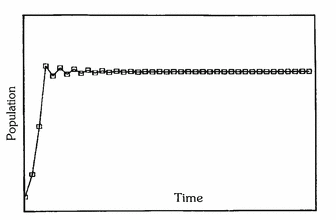
\includegraphics[width = 0.6\textwidth]{img/r1_8.png}
\caption{Evolución de la población con $r=1.8$}
\label{fig:r1_8}
\end{figure}

Para $r>2$, la ecuación anterior predice un crecimiento de la desviación lo que nos permite deducir que el punto fijo $x_0=1$ resulta ser inestable. Las figura \ref{fig:r2_3}, \ref{fig:r2_5} y \ref{fig:r3} muestran la evolución de la población para valores de $r$ en la región inestable.

\begin{figure}[hbtp]
\centering
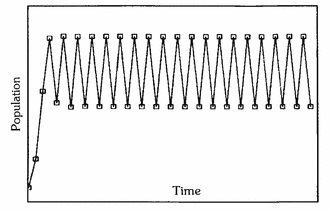
\includegraphics[width = 0.6\textwidth]{img/r2_3.png}
\caption{Evolución de la población con $r=2.3$}
\label{fig:r2_3}
\end{figure}
\begin{figure}[hbtp]
\centering
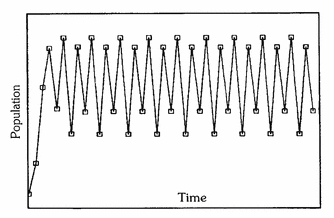
\includegraphics[width = 0.6\textwidth]{img/r2_5.png}
\caption{Evolución de la población con $r=2.5$}
\label{fig:r2_5}
\end{figure}
\begin{figure}[hbtp]
\centering
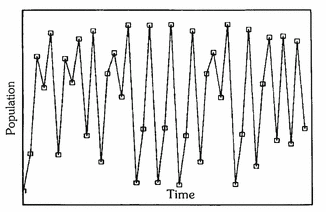
\includegraphics[width = 0.6\textwidth]{img/r3.png}
\caption{Evolución de la población con $r=3$}
\label{fig:r3}
\end{figure}

\subsection{Conjuntos de Julia y Mandelbrot}

\subsubsection{Repaso de números complejos}
Antes de comenzar a hablar de los fractales de Julia y Mandelbrot se hace necesario dar una pequeña referencia sobre los números complejos. Básicamente podemos definir un número complejo como una expresión de la forma:
\[z=a +bi\]
Donde a y b son numeros reales, e i es la raíz cuadrada de -1.

Los números complejos se representan en un plano: \textbf{el plano complejo}, de manera que cada número complejo tiene asociado un punto del plano y viceversa. Es en esta identificación entre puntos del plano y números complejos en lo que se basa la representación de los fractales.

\subsubsection{Conjunto de Julia}
\begin{definition}[Conjunto de Julia]
Los \textbf{conjuntos de Julia}, así llamados por el matemático Gaston Julia, son una familia de conjuntos fractales que se obtienen al estudiar el comportamiento de los números complejos al ser iterados por una función.

Son conjuntos de Julia, por ejemplo, los formados por la familia cuadrática definida poeqr la ecuación de recurrencia vista en el ejemplo \ref{example:Julia}:

\begin{equation}\label{eq:Julia}
z_{n+1} = z_n^2+c \text{ siendo } c \text{ un número complejo}
\end{equation}

\end{definition}

Para explicar los conjuntos de Julia nos basaremos en el ejemplo que acabamos de comentar, aunque puede realizarse una construcción equivalente con muchas otras funciones.

El conjunto de Julia que se obtiene a partir de esta función se denota \textbf{J$_c$}. Para construirlo, partiendo de un punto cualquiera $z_0$, aplicamos la ecuación \eqref{eq:Julia} de manera iterativa obteniendo una serie de puntos del plano:
\[\begin{array}{l}
z_0=z_0\\
z_1=z_0^2+c \\
z_2 = z_1^2 + c \\
\vdots \\
z_{n+1} = z_n^2+c
\end{array}\]

Si esta sucesión queda acotada, entonces se dice que $z$ pertenece al conjunto de Julia de parámetro $c$, denotado por $J_c$; de lo contrario, si la sucesión tiende al infinito, $z$ queda excluido de éste.

Debido a la enorme cantidad de cálculos que se necesitaban para obtener la gráfica correspondiente, se tuvo que esperar hasta los años ochenta para poder representar estos conjuntos.

Algunos ejemplos de conjuntos de Julia aplicando diferentes valores de $c$ a la ecuación anterior están representados en la figura \ref{fig:Julia}

\begin{figure}[hbtp]
\centering
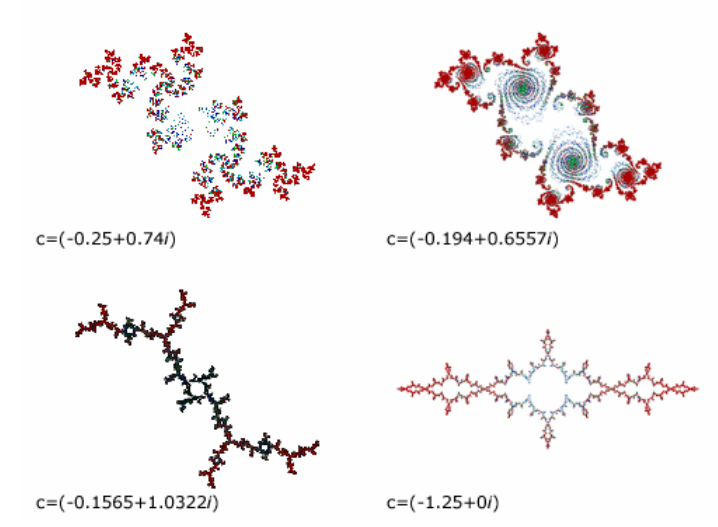
\includegraphics[width = 0.6\textwidth]{img/Julia_sets.png}
\caption{Ejemplos de conjuntos de Julia}
\label{fig:Julia}
\end{figure}

Puede demostrarse que si $|z_n| > 2$ entonces la sucesión diverge y el punto $z_0$ no pertenece al conjunto de Julia. Por lo tanto, basta encontrar un sólo término en la sucesión que verifique esta desigualdad para tener la certeza de que $z_0$ no está en el conjunto.

\subsubsection{Conjunto de Mandelbrot}
\begin{definition}
El conjunto de Mandelbrot es el más conocido de los conjuntos fractales y el más estudiado. Se conoce así en honor al matemático Benoît Mandelbrot (1924-2010), que investigó sobre él en los años setenta.

Mandelbrot modifica el proceso iterativo de Julia haciendo variable el punto $c$ y fijando el punto $z_0=0$. El conjunto de Mandelbrot es el conjunto de números complejos $c$ para los cuales la sucesión de puntos obtenida por el método iterativo:
\[\begin{array}{l}
z_0=z_0\\
z_1=z_0^2+c \\
z_2 = z_1^2 + c \\
\vdots \\
z_{n+1} = z_n^2+c
\end{array}\]
no tiende a infinito, es decir, está acotada.
\end{definition}

La figura \ref{fig:Mandelbrot} muestra la representación del conjunto de Mandelbrot obtenida si asignamos el color negro a los puntos $c$ que dan lugar a sucesiones acotadas y otros colores a los demás puntos, según lo rápido que tiendan al infinito.

\begin{figure}[hbtp]
\centering
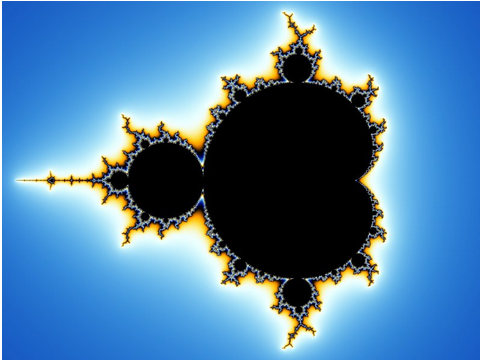
\includegraphics[width = 0.6\textwidth]{img/Mandelbrot_set.png}
\caption{Conjunto de Mandelbrot}
\label{fig:Mandelbrot}
\end{figure}

Si la constante $c$ fuera la misma para todos los puntos del dibujo y no dependiera de la posición, obtendríamos los anteriores conjuntos de Julia. Hay uno diferente para cada punto del plano complejo. Por tanto, estos conjuntos están completamente relacionados con el conjunto de Mandelbrot. Para cada punto de éste se puede decir que hay un conjunto de Julia. La figura \ref{fig:Mandelbrot-Julia} ilustra esta relación:

\begin{figure}[hbtp]
\centering
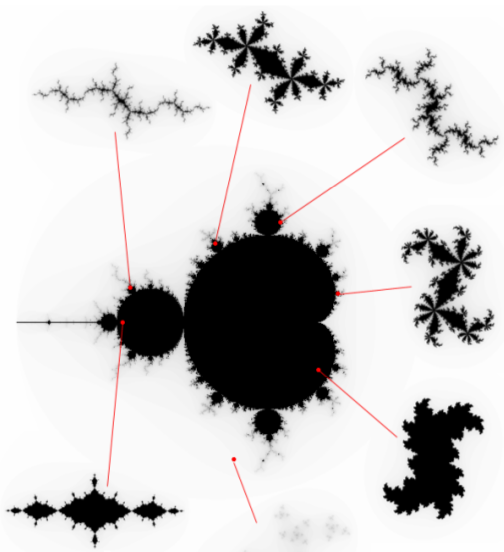
\includegraphics[width = 0.6\textwidth]{img/Mandelbrot-Julia.png}
\caption{Conjuntos de Julia asociados a cada punto del conjunto de Mandelbrot}
\label{fig:Mandelbrot-Julia}
\end{figure}

Queda claro pues que los conjuntos de Mandelbrot y Julia están estrechamente relacionados. El conjunto de Mandelbrot itera $z=z^2+c$ comenzando con $z = 0$ y variando el valor de $c$. El de Julia, por su parte, itera esa misma función, pero con valores fijos para $c$ y variando los de $z$. Cada punto $c$ en el conjunto de Mandelbrot especifica la estructura geométrica del conjunto de Julia correspondiente. Si $c$ está en el conjunto de Mandelbrot, entonces el de Julia será conectado (cerrado). De lo contrario, el conjunto de Julia será sólo una colección de puntos desconectados, trazados sobre una gráfica.

\subsection{Fractales, dimensión de Hausdorff y dimensión fractal}

El término fractal fue propuesto por el matemático \textbf{Benoit Mandelbrot} en 1975, procedente del latin ``Fractus'' que significa ``fracturado''.

El fractal más famoso, si cabe, se debe a Mandelbrot quien lo obtuvo analizando la famosa ecuación en complejos
\[x_{n+1} = x_n^2 + c\]
estudiada en la sección anterior.

Recordemos que en la figura \ref{fig:Mandelbrot} la diferencia entre los distintos colores mostrados se debía a la convergencia o no de los diferentes puntos del plano al aplicarles la ecuación de Mandelbrot.

Aquí se encuentra la relación entre el caos y los fractales. Si se tratase de una figura ``normal'' los puntos que convergen son los de color negro y los de color azul los que no. De esta forma podríamos tener el resultado de la ecuación ``controlado''.

Sin embargo, cuando nos acercamos a la ``frontera'' del dibujo volvemos a observar la misma figura con lo que la frontera no está tan clara. Si repetimos el proceso volvemos a la misma situación inicial. Podríamos ``hacer zoom'' \emph{infinitamente} y seguiríamos observando figuras similares.

\subsubsection{Fractales en la vida real}
Puede parecer que los fractales no son más que un artificio matemático para representar el comportamiento de ecuaciones artificiales pero nada más lejos de la realidad. \emph{Los fractales están muy prsentes en la vida diaria}, como muestran las figuras \ref{fig:concha} y \ref{fig:brocoli}

\begin{figure}[hbtp]
\centering
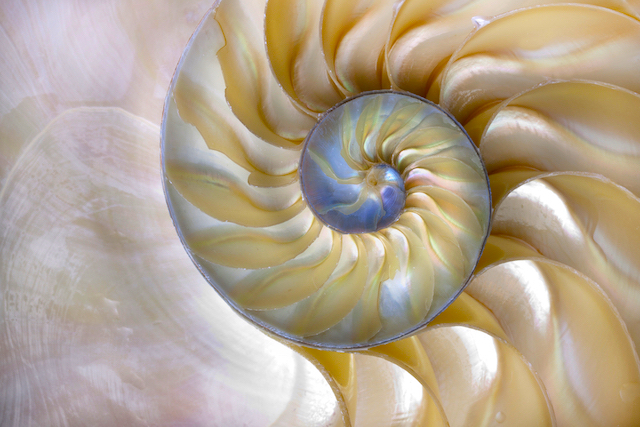
\includegraphics[width = 0.6\textwidth]{img/concha.jpg}
\caption{Concha de un molusco}
\label{fig:concha}
\end{figure}

\begin{figure}[hbtp]
\centering
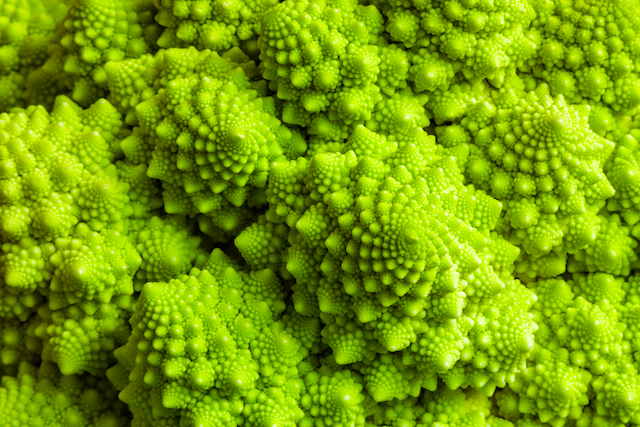
\includegraphics[width = 0.6\textwidth]{img/brocoli.jpg}
\caption{Trozo de brocoli al que se ha aplicado zoom}
\label{fig:brocoli}
\end{figure}

La existencia de los fractales en la vida cotidiana se debe a la gran capacidad de comprimir información que tienen asociada. Así, por ejemplo, un árbol puede ser un ejemplo de fractal donde cada rama ``se comporta como un pequeño árbol'' del que crecen ramas de las que crecerán otras ramas... hasta llegar a las hojas.

Obviamente los fractales que se encuentran en la vida real son finitos pues al final todo se compone de células pero la idea que hay detrás de este tipo de formaciones es la de fractal.

Como explicaremos en la sección \ref{sec:compresionFractal} nos hemos ayudado de esta capacidad de comprimir información para desarrollar diferentes técnicas de compresión.

\subsubsection{Dimensión de Hausdorff y dimensión fractal}
\begin{definition}[Dimensión de Hausdorff]
La \textbf{dimensión de Hausdorff} o dimensión de Hausdorff-Besicovitch es una generalización métrica del concepto de dimensión de un espacio topológico, que permite definir una dimensión fraccionaria (no entera) para un objeto fractal.
\end{definition}

Mejor que introducir la definición formal de dimensión topológica, demos una definición intuitiva. La \textbf{dimensión topológica} de un cierto objeto en un espacio es $d$ si y sólo si cada punto del objeto se puede \emph{desconectar} (es decir, quitar uno o varios puntos dejando el objeto inconexo) del resto por un conjunto de dimension $d-1$. Es decir, curvas y círculos pueden ser desconectados quitando puntos cualesquiera aislados (por tanto, tienen dimensión topológica 1, que es la dimensión de un punto: 0, más 1); las esferas pueden ser desconectadas quitando curvas o circunferencias de la misma (por tanto tienen dimensión 2) y así sucesivamente.

Todas estas dimensiones son enteras (hay dimensiones infinitas pero podemos prescindir de ellas para lo que nos interesa). Sin embargo, la dimensión topológica es a veces algo \emph{bruta}, en el sentido de que los fractales, por ejemplo, tienen dimensión topológica entera pero, en términos del espacio que ocupan, se comportan como objetos de dimensión mayor.

Es por ello conviene precisar un nuevo concepto de dimensión: \textbf{dimensión de Hausdorff}. De nuevo, intuitivamente, la dimensión de Hausdorff nos dice cómo el objeto en cuestión llena el espacio en el que está inmerso. Para ellos recubriremos la figura con \emph{bolas} de radio $r$. La razón entre el número de bolas que necesitemos $N(r)$ y $ln(\frac{1}{r})$ es la dimensión fractal de nuestro objeto. Esto es,

\begin{equation}
D = \frac{N(r)}{ln(\frac{1}{r})}
\end{equation}

En particular, la dimensión topológica de un fractal es siempre estrictamente menor que su dimensión de Hausdorff.

\subsubsection{Ejemplos}
La figura \ref{fig:gb} muestra la dimensión fractal de la isla de Gran Bretaña.
\begin{figure}[hbtp]
\centering
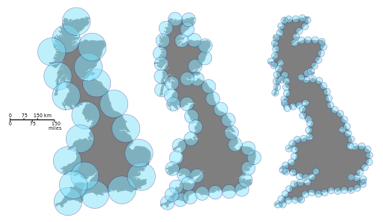
\includegraphics[width = 0.6\textwidth]{img/GB.png}
\caption{Medida fractal de la línea de costa de Gran Bretaña}
\label{fig:gb}
\end{figure}

Otros ejemplos de objetos con dimensión fractal se muestran en la tabla \ref{tab:ejemplos}.

\begin{figure}[hbtp]
\footnotesize
\begin{tabular}{ |c|c|c|}
  \hline
  \textbf{Valor exacto} & \textbf{Valor aproximado} & \textbf{Nombre} 	\\\hline
  $\frac{log(2)}{log(3)}$ & 0.6309 & Conjunto de Cantor \\
  Medida (recuento de cajas) & 1,2 & Conjunto de Julia \emph{Dendrita} \\
  $\frac{log(\frac{1+\sqrt[3]{73-6\sqrt{87}}+\sqrt[3]{73+6\sqrt{87}}}{3})}{log(2)}$ & 1,5236 & Frontera de la curva Dragón \\
  $3\frac{log(\phi)}{log(1+\sqrt{2})}$ & 1,6379 & Fractal de Fibonacci \\
  2 & 2 & Frontera del Conjunto de Mandelbrot \\
  Medido & 1,24 & Línea de costa de Gran Bretaña \\
  Medido & 1,52 & Línea de costa de Noruega \\
  \hline
\end{tabular}
\normalsize
\caption{Ejemplos de conjuntos con dimensión fractal}
\label{tab:ejemplos}
\end{figure}

\subsection{Polvo de Cantor}

\begin{definition}[Polvo de Cantor]
Se denomina Polvo de Cantor al fractal resultante de iterar sobre el conjunto de cantor en dos dimensiones.
\end{definition}

\begin{definition}[Conjunto de Cantor]
El conjunto de Cantor, llamado así por ser aporte de Georg Cantor en 1883, se construye de la siguiente manera:

En un primer paso tomamos el intervalo [0,1], lo dividimos en 3 intervalos iguales y eliminamos el intervalo central, por lo que nos quedarían 2 intervalos nuevos [0,1/3] y [2/3,1].

Tras esto, repetimos el mismo proceso con cada uno de los intervalos resultantes con lo que nos quedarían los siguientes intervalos: [0,1/9] , [2/9,1/3] , [2/3,7/9] , [8/9,1]. Y así sucesivamente.

La imagen \ref{fig:conjuntoCantor} ilustra la construcción de este conjunto.
\end{definition}

\begin{figure}[hbtp]
\centering
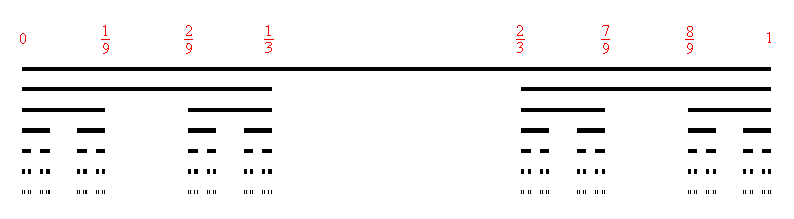
\includegraphics[width = 0.6\textwidth]{img/conjuntoCantor.png}
\caption{Primeras etapas del proceso de construcción del conjunto de Cantor}
\label{fig:conjuntoCantor}
\end{figure}

El conjunto de Cantor exhibe de forma evidente una de las propiedades más importantes de los fractales: la autosimilaridad. Ya que conforme se van aumentando las iteraciones se puede observar de nuevo el conjunto de cantor original.

Como curiosidad se le denominó Polvo de Cantor porque una vez iterado el conjunto, un número determinado de veces los segmentos se hacen cada vez mas pequeños semejando puntos luciendo como una fila de partículas de polvo dispuestas con regularidad fractal.

%%%%%%%%%%%%%%%%%%%%%%%%%%%%%%%%%%%%%%%%%%%%%%%%%%%%%%%%%%
%%%%%%%%%%%%%%%%%%%%%%%%%%%%%%%%%%%%%%%%%%%%%%%%%%%%%%%%%%
%%%%%%%%%%%%%%%%%%%%%%%%%%%%%%%%%%%%%%%%%%%%%%%%%%%%%%%%%%
%%%%%%%%%%%%%%%%%%%%%%%%%%%%%%%%%%%%%%%%%%%%%%%%%%%%%%%%%%
%%%%%%%%%%%%%%%%%%%%%%%%%%%%%%%%%%%%%%%%%%%%%%%%%%%%%%%%%%
%%%%%%%%%%%%%%%%%%%%%%%%%%%%%%%%%%%%%%%%%%%%%%%%%%%%%%%%%%
%%%%%%%%%%%%%%%%%%%%%%%%%%%%%%%%%%%%%%%%%%%%%%%%%%%%%%%%%%
%%%%%%%%%%%%%%%%%%%%%%%%%%%%%%%%%%%%%%%%%%%%%%%%%%%%%%%%%%
%%%%%%%%%%%%%%%%%%%%%%%%%%%%%%%%%%%%%%%%%%%%%%%%%%%%%%%%%%

\section{Sistemas continuos}
% Tiempo estimado de esta parte: 70 min.\\
% Referencia
% \begin{itemize}
% \item CHAOS: An introduction to dynamical systems temas 7,8,9 y 11.
% \item Elegant Chaos
% \end{itemize}

\subsection{Sistemas dinámicos deterministas, ecuaciones diferenciales}

Los sistemas dinámicos continuos deterministas, definidos en \ref{def:sistemaDinamico}, vienen modelizados por ecuaciones diferenciales.

En lugar de expresar el estado actual en función de un estado anterior, las ecuaciones diferenciales tratan de expresar la \emph{tasa de cambio} del estado actual en función del estado actual. La tasa de cambio de una cierta función es su \emph{derivada}. Tenemos la siguiente definición general de ecuación diferencial.

\begin{definition}[Ecuación diferencial]
Una ecuación diferencial es una fórmula matemática que relaciona una función con sus derivadas.
\end{definition}

\begin{example}[Ecuación del calor]\label{ex:calor}
Un ejemplo de este tipo de dependencia es la \emph{Ley del calor de Newton}. Si consideramos $x$ como la diferencia de temperatura entre el objeto caliente y la temperatura ambiente del aire que lo rodea, la tasa de cambio de esta diferencia de temperatura es inversamente proporcional a la diferencia de temperatura. En términos de ecuaciones diferenciales, diremos:
\begin{equation}
x'(t) = ax(t)~~~con~~ a<0
\end{equation}

La solución de esta ecuación viene dada por:
\begin{equation}
x(t) = c\cdot e^{at}
\end{equation}

Esto quiere decir que la diferencia de temperatura $x(t)$ decrece exponencialmente con el tiempo $t$. Se trata de una ecuación  de \emph{primer orden}, puesto que el \emph{orden} de la derivada más alto que aparece es el de la \emph{primera} derivada, y \emph{lineal} porque la relación entre las funciones $x'(t)$ y $x(t)$ en la ecuación es \emph{lineal}.
\end{example}

En el siguiente ejemplo, veremos un caso de ecuación diferencial \emph{de segundo orden} \emph{no lineal}.

\begin{example}[Péndulo]
En este caso estudiaremos el movimiento de un péndulo \emph{bob}, el movimiento de un péndulo que tiene en su extremo un peso y que cuelga de un soporte que limita su movimiento a lo largo de un círculo. La aceleración que experimenta este péndulo es tangente a la dirección del movimiento y proporcional a la componente de la fuerza gravitatoria sobre la dirección tangencial. Si representamos con $x(t)$ la posición angular (es decir, la razón entre la longitud del arco que forma el péndulo con la vertical y la longitud del péndulo), entonces la relación entre su derivada segunda y ésta viene dada por:
\begin{equation}
x''(t) = -\sin x(t)
\end{equation}

Esta ecuación es una de las más importantes en ciencia y se trata de una ecuación de \emph{segundo orden}, puesto que el \emph{orden} de la derivada más alto que aparece es el de la \emph{segunda} derivada, y \emph \emph{no lineal}, porque la relación entre las funciones $x''(t)$ y $x(t)$ en la ecuación es \emph{no lineal}.
\end{example}


En ambos ejemplos, buscamos soluciones de la forma $x(t)$ donde $t$ denota el tiempo y $x(t)$, por tanto, una cierta magnitud física que varía en función del tiempo: en el primer ejemplo, la diferencia de temperatura; en el segundo ejemplo, la posición angular. Es por eso que consideramos que $x(t)$ es una variable \emph{dependiente}.


\begin{definition}[Ecuación diferencial autónomas]
Si la variable \emph{independiente} $t$ no aparece explicítamente en la ecuación, como es el caso en los dos ejemplos anteriores, hablaremos de ecuaciones diferenciales \textbf{autónomas}. Si $t$ aparece explícitamente en la ecuación como es el caso de la ecuación del \emph{péndulo amortiguado} (el columpio):
\begin{equation}
x''(t) = -cx'(t)-\sin x(t)+\rho~\sin t
\end{equation}
entonces hablaremos de ecuaciones diferenciales \textbf{no autónomas}.
\end{definition}

Recapitulando las nociones vistas hasta ahora tendríamos la siguiente clasificación de las ecuaciones diferenciales:

\begin{itemize}
\item Según el orden de las derivadas que aparezcan en la expresión:
	\begin{itemize}
	\item Primer orden
	\item Segundo orden
	\item ...
	\end{itemize}
\item Según la relación entre la función $x$ y sus derivadas
	\begin{itemize}
	\item Lineales
	\item No lineales
	\end{itemize}
\item Según si aparece explicítamente la variable $t$ en la ecuación
	\begin{itemize}
	\item Autónomas
	\item No autónomas
	\end{itemize}
\end{itemize}

Si recuperamos el ejemplo \ref{ex:calor}, teníamos que las soluciones eran de la forma:
\begin{equation}
x(t) = c \cdot e^{at}
\end{equation}

La $c$ es una constante en $\mathbb{R}$, cuyo valor dependerá del punto inicial que tomemos, es decir, la ecuación diferencial planteada en \ref{ex:calor} tiene \emph{infinitas} soluciones, a menos que especifiquemos un \emph{valor inicial} $x(0)$.

En el momento en que definimos un valor inicial $x(0)=x_0$ tenemos:
\[x(0)=c\cdot e^0=c \implies c=x_0 \implies x(t) = x(0)\cdot e^{at}\]

Así, estamos \emph{seleccionando} una de las soluciones dentro de la familia de soluciones.


% No se que aparece en la pagina que decías, pero yo me dibujo aquí la familia de funciones que creo que hay que poner xd
\begin{center}
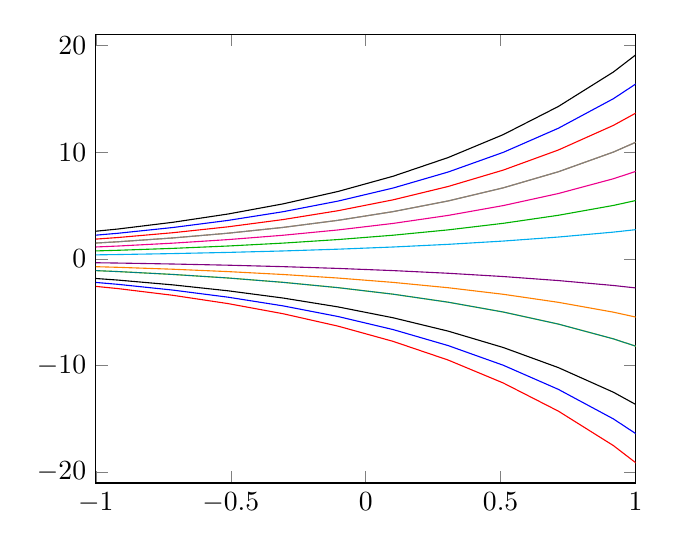
\begin{tikzpicture}
\begin{axis}[xmin=-1, xmax=1, samples=50, cycle list name=color list]
  \addplot (x,-7*e^x);
  \addplot (x,-6*e^x);
  \addplot (x,-5*e^x);
  \addplot (x,-3*e^x);
  \addplot (x,4*e^x);
  \addplot (x,-3*e^x);
  \addplot (x,-2*e^x);
  \addplot (x,-1*e^x);
  \addplot (x,e^x);
  \addplot (x,2*e^x);
  \addplot (x,3*e^x);
  \addplot (x,4*e^x);
  \addplot (x,5*e^x);
  \addplot (x,6*e^x);
  \addplot (x,7*e^x);
\end{axis}
\end{tikzpicture}
\captionof{figure}{Familia de funciones de la forma $x(t)=x(0)e^t$}
\end{center}

En nuestro caso, podemos establecer:

\begin{equation}
x(0) = x_0
\end{equation}

y por tanto, la solución particular de nuestro problema sería:

\begin{equation}
x(t) = x_0e^{at}.
\end{equation}

En general, a los problemas experesados en forma de ecuación diferencial más dato inicial, los denominaremos \textbf{problemas de valor inicial}.\newline
Es el momento de introducir el concepto de \emph{espacio de fases}, que nos permitirá estudiar el comportamiento cualitativo de nuestras soluciones, e incluso, será la idea a la que nos aferremos para obtener las soluciones en casos más complicados.

\subsection{Espacio de estados/fases}

Un concepto muy útil a la hora de trabajar con ecuaciones diferenciales son los \textbf{diagramas de fases}, pues nos permite conocer de manera inequívoca el estado de nuestra sistema en cualquier tiempo futuro.

Tomemos la ecuación diferencial
\[y(x)'=f(y(x))\]
donde la función $f$ viene dada por la siguiente gráfica

\begin{figure}[hbtp]
\centering
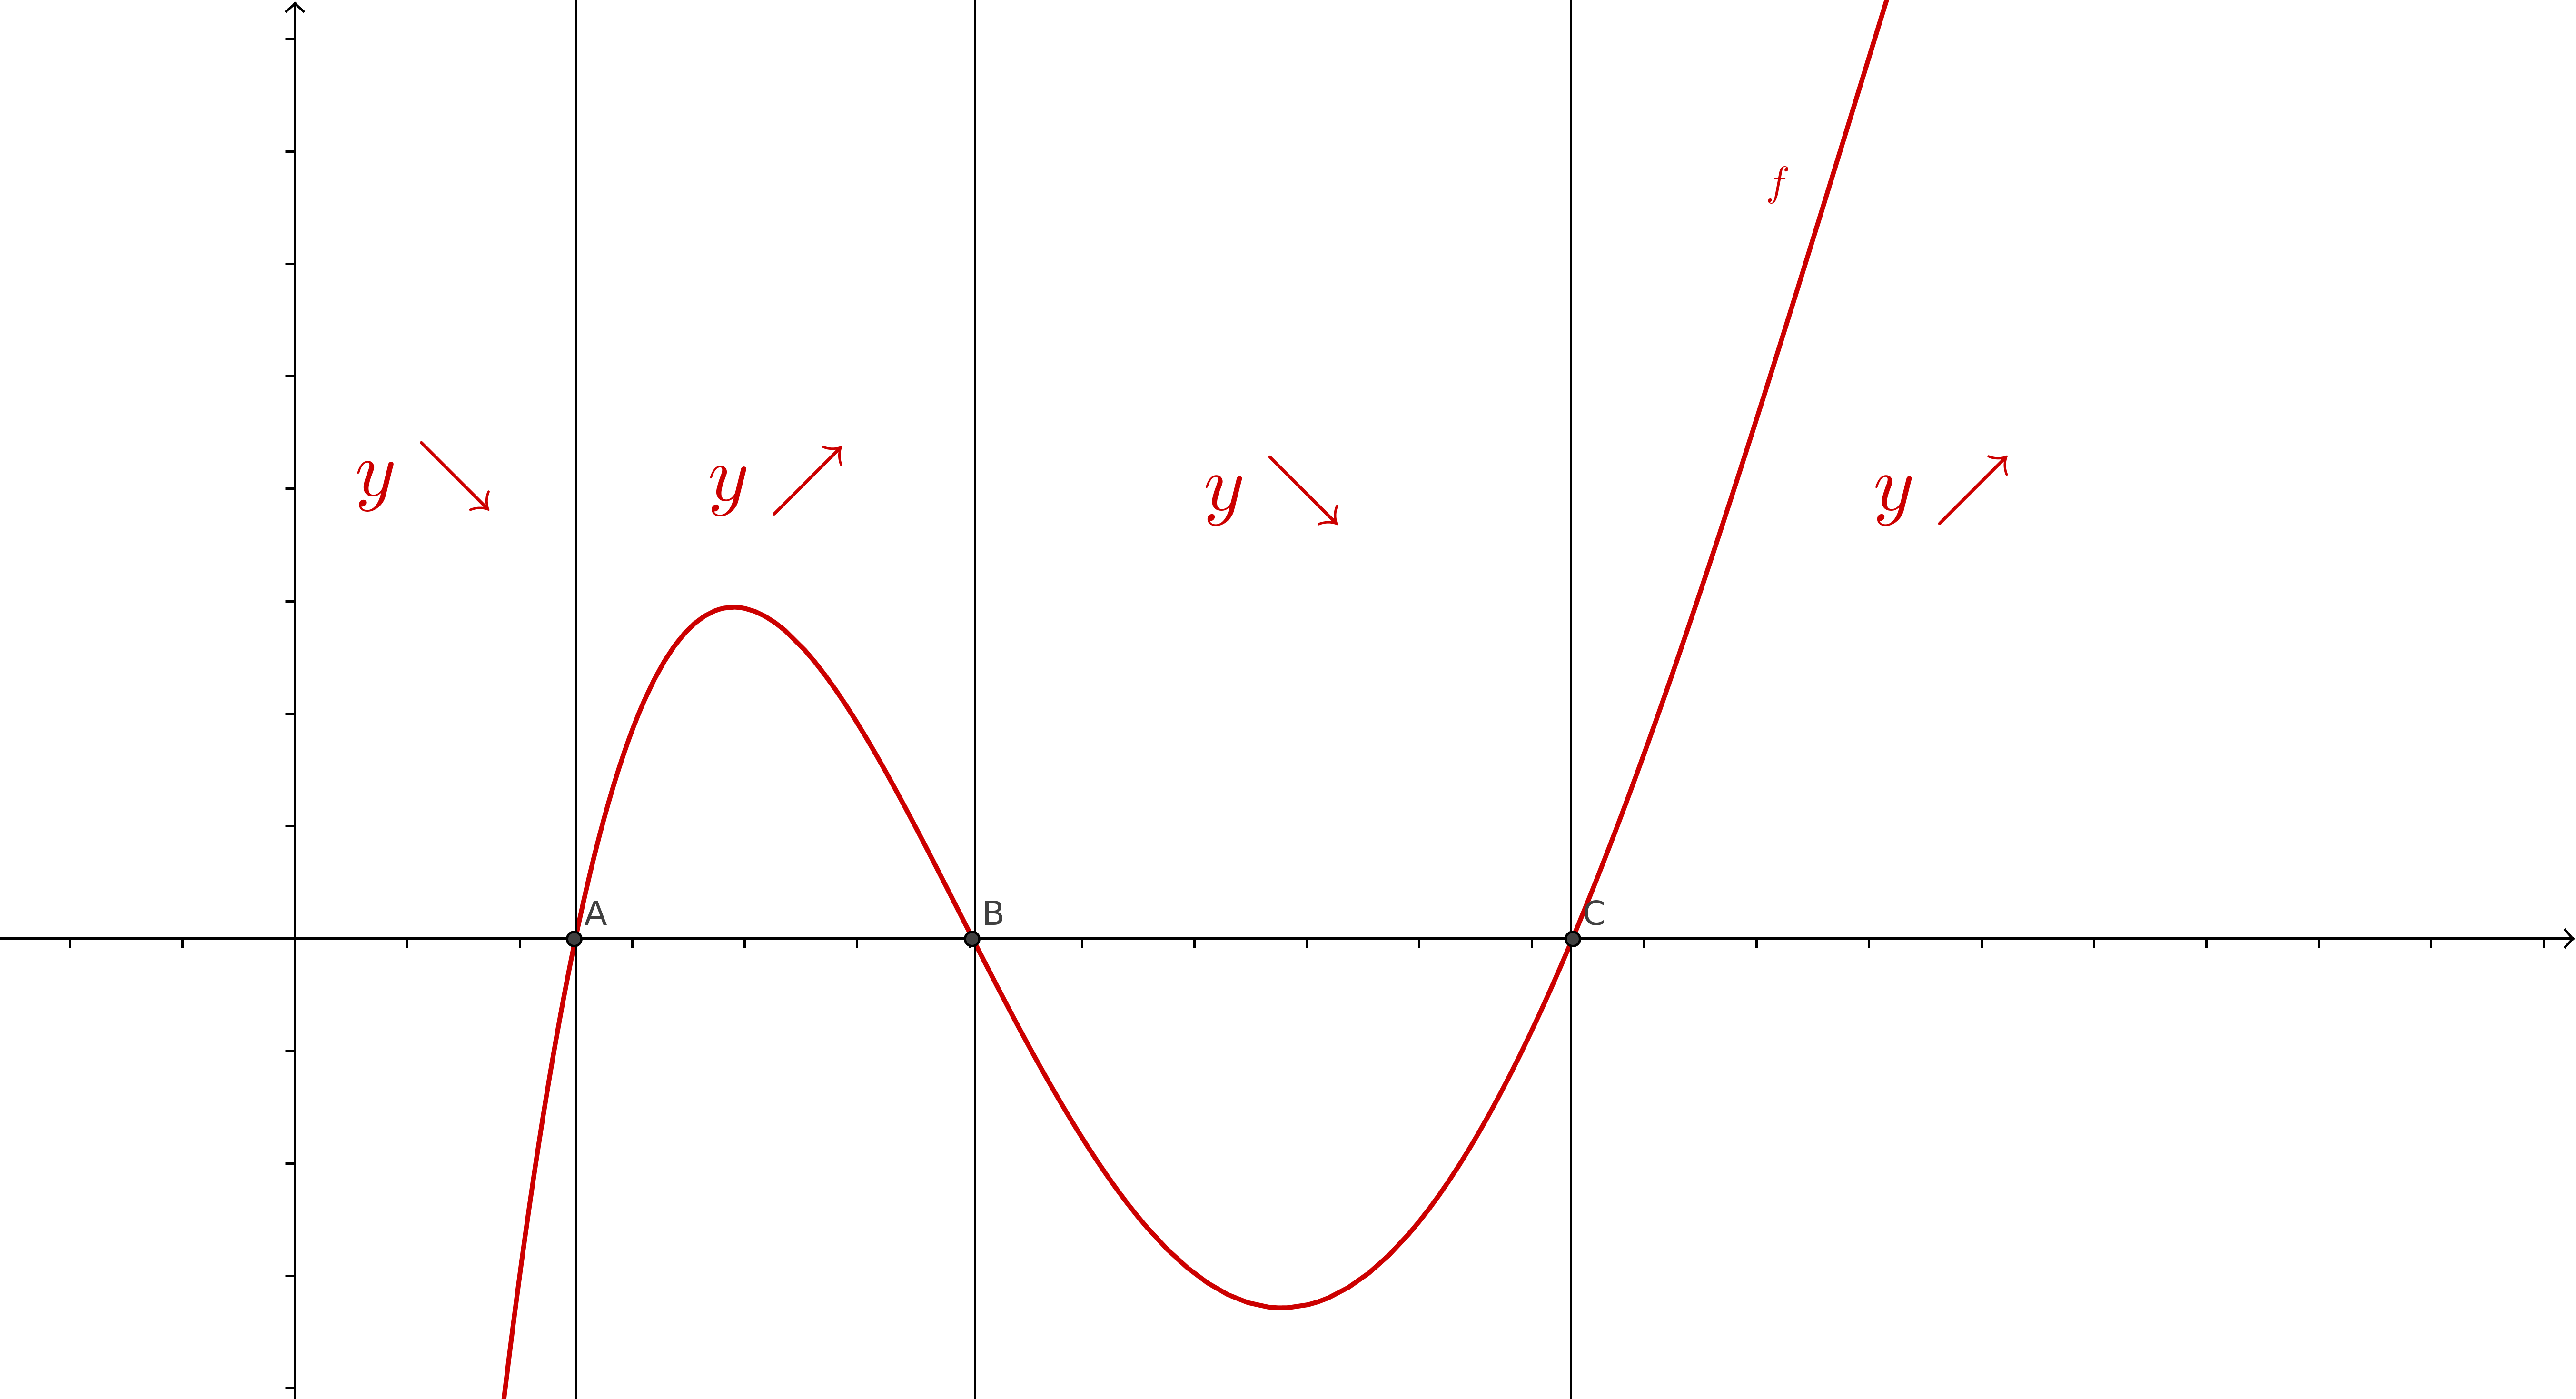
\includegraphics[width = 0.6\textwidth]{img/propiedades-autonomas.png}
\end{figure}

Podemos observar que si nos situamos ``a la izquierda de $a$'' o ``entre $b$ y $c$'' la función $y$ es decreciente. Del mismo modo, si nos situamos ``entre $a$ y $b$'' o ``a la derecha de $c$'' la función será creciente mientras que en los puntos $a, b$ y $c$ la función ni crece ni decrece. Esta información queda recogida en el siguiente diagrama de fases:

\begin{figure}[hbtp]
\centering
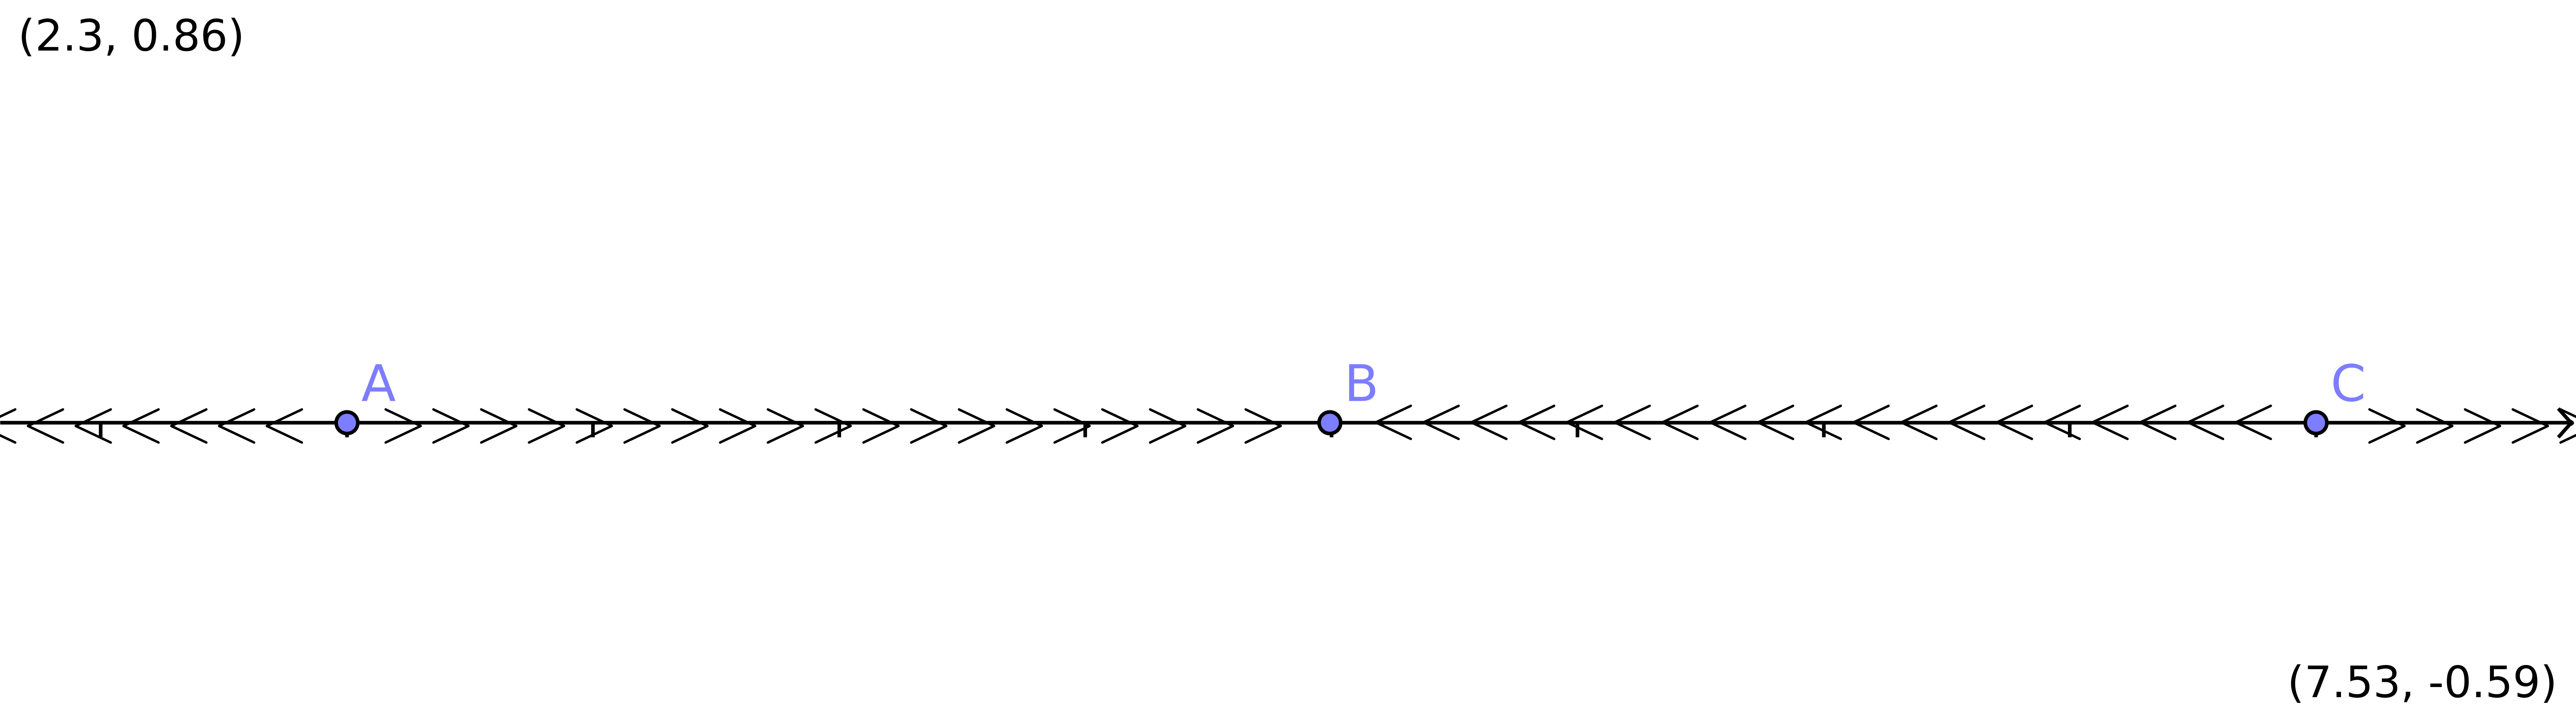
\includegraphics[width = 0.6\textwidth]{img/diagrama-fases.png}
\end{figure}

En este caso diremos que $a$ y $c$ son puntos \textbf{inestables} pues una pequeña perturbación hará que nos alejemos de ellos. Igualmente, diremos que $b$ es un punto \textbf{estable} porque una pequeña perturbación hará que volvamos de nuevo a desplazarnos hacia $b$.

\begin{example}
Retomamos el ejemplo \ref{ex:calor} considerando un valor $a=-1$. Ya vimos que la solución a la EDO (ecuación diferencial de primer orden) era:
\[x(t) = x(0)\cdot e^{-t}\]

En esta ocasión, estudiando el signo de la derivada $x'(t)=ax(t)$ vemos que la pendiente sólo se anula en $x(t)=0$ y que una vez que la función $x(t)$ toma un valor positivo empieza a decrecer del mismo modo que crece al encontrar un valor negativo. Por tanto tenemos un punto estable en $x(t)=0$. Esto provoca que un pequeño error en la aproximación del dato inicial, cuanto tomamos $t$ grande, no nos aleje mucho del valor real.

Es decir, si tomamos por error $\tilde{x}_0 = x_0 + ε$, estamos cometiendo un error ε en la medida del dato inicial, lo que nos lleva a un error:
\[x(t)-\tilde{x}(t) = x_0\cdot e^{-t} - \tilde{x}_0\cdot e^{-t} = e^{-t}\cdot ε\]
al evaluar la función. Puesto que tenemos una exponencial en el denominador, por mucho error ε que hayamos cometido, al final, este será ``despreciable''.
\end{example}

\begin{example}
Repitamos el mismo ejemplo con $a=1$. En este caso tendremos:
\[x(t) = x(0)\cdot e^{t}\]

Imitando el ejemplo anterior es trivial comprobar que no hay ningún punto estable.

Por tanto, si tomamos por error $\tilde{x}_0 = x_0 + ε$, estamos cometiendo un error ε en la medida del dato inicial, lo que nos lleva a un error:
\[x(t)-\tilde{x}(t) = x_0\cdot e^{t} - \tilde{x}_0\cdot e^{t} = e^{t}\cdot ε\]
al evaluar la función. Puesto que tenemos una exponencial el error cometido se dispara.
\end{example}

\subsection{Sistemas de ecuaciones no lineales}
Hasta ahora la tarea ha sido relativamente sencilla, sin embargo, no podemos decir lo mismo cuando estudiamos sistemas dinámicos \emph{no lineales}. La mayoría de los sistemas no lineales de ecuaciones diferenciales no pueden ser resueltos de manera explícita, es decir, las soluciones a dicho sistema no se pueden obtener mediante cálculo. Usaremos métodos geométricos que nos revelarán propiedades cualtitativas de las soluciones: Para qué valores del dato inicial las soluciones son crecientes? Para qué valores son decrecientes?,...

Utilicemos un ejemplo para ilustrar los conceptos siguientes: Supongamos que trabajamos con un modelo para estudiar la evolución de una cierta población. Es común, en este caso, utilizar la función \emph{logística} de la población:

\begin{equation}
x'(t) = a\cdot x(t)(1-\frac{x(t)}{K})~~~~con~~a>0~~y~~K>0
\end{equation}
A esta ecuación la llamamos \emph{ecuación diferencial logística}. En ese caso, $x(t)$ mide la población de una cierta especie. Llamamos $K$ al valor de la población \emph{limitante}, aquel a partir del cual la población deja de crecer y, de hecho decrece, por sobrepoblación.

Este tipo de comportamiento solo puede ser modelado mediante una ecuación no lineal. Ahora nos preguntamos: Es posible predecir para qué valores iniciales la población crecerá? Y para que valores sólo decrecerá?

En la figura \ref{fig:poblacion} observamos las soluciones de la ecuación diferencial logística.

\begin{figure}[hbtp]
\centering
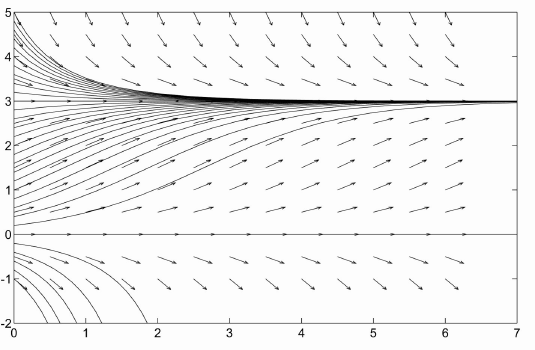
\includegraphics[width = 0.6\textwidth]{img/poblacion.png}
\caption{Soluciones de la ecuación logística diferencial}
\label{fig:poblacion}
\end{figure}


Con lo que hemos visto sobre puntos estables e inestables, le resultará sencillo al lector detectar que en $x=1$ tenemos un punto estable, mientras que en $x=0$, tenemos un punto inestable. Decimos que ambas soluciones $x(t) = 0$ y $x(t) = 1$ son \textbf{soluciones de equilibrio}.

Ahora podemos resolver las preguntas planteadas anteriormente. La población crecerá siempre que la población sea positiva y estrictamente menor que $K$. Mientras que decrecerá siempre que sea superior a $K$. Por otro lado, las soluciones que corresponden con valores negativos de la población y que \emph{explotan} (se van a infinito) en tiempo finito, afortunadamente, pueden descartarse pues no tienen sentido físico.\newline

Para poder resolver sistemas de ecuaciones a partir de sus gráficas, nos basamos en los siguientes 3 conceptos importantes:

\begin{itemize}
\item \textbf{Existencia de solución} Para cada punto $(t,x)$ de la gráfica existe una  solución $x(t)$ que pasa por ese punto. La pendiente de dicha solución viene dada por la ecuación diferencial en ese punto.
\item \textbf{Unicidad de la solución} Para cada punto $(t,x)$ de la gráfica únicamente pasa una solución.
\item \textbf{Dependencia continua} Dada una cierta solucion $x(t)$ para un cierta condición inicial, las soluciones próximas en un cierto entorno del dato inicial permanecen próximas a lo largo de intervalos cortos de tiempo.
\end{itemize}

El concepto de dependencia continua no debe ser confundido con el de dependencia \emph{sensible} de las condiciones iniciales, también conocido como \textbf{efecto mariposa}. Éste hace refencia a la propiedad de ciertos sistemas dinámicos no lineales en los que una pequeña variación en los datos iniciales resulta en grandes variaciones en estados futuros tras un largo período de tiempo. Esta es la característica más importante de los \textbf{sistemas caóticos}.

%\subsection{Oscilaciones}
%
%\begin{definition}[Ecuación diferencial oscilante]
%Decimos que una ecuación diferencial es oscilante cuando tiene infinitos puntos críticos. Un ejemplo de ecuación de este tipo es
%\[x''(t)+x(t)=0\]
%de la que $x(t)=\sin(t)$ es una solución.
%\end{definition}
%
%Con este tipo de ecuaciones nos encontramos con que hay numerosos puntos de estabilidad.
%
%Sabemos que un pequeño error respecto al dato inicial, si este era el único punto estable, no era un problema puesto que la solución se acababa aproximando bastante a la estabilidad.
%
%No obstante, si tenemos varios puntos de estabilidad la duda que nos surge es, ¿De qué solución real no se distancia mucho el valor que calculemos?

\subsection{Sistemas disipativos: atractores}
Los sistemas dinámicos procedentes de las aplicaciones físicas tienden a ser \textbf{disipativos}: debido a alguna fuerza externa, el movimiento cesa. Esta disipación puede venir de fuerzas de fricción, pérdidas termodinámicas,... Debido a este efecto, el sistema entra en su comportamiento típico en una región en la que se da una condición local de mínima energía. Si observaramos el espacio de fases del sistema distingiríamos una parte a la que las trayectorias se aproximan y que permanece invariante a largo plazo.

De manera informal un \textbf{atractor} es un conjunto hacia el que todas las trayectorias cercanas convergen. Los puntos fijos y los ciclos estables son ejemplos de atractores.

\begin{definition}[Atractor]
Un atractor es un conjunto cerrado, $A$, con las siguientes propiedades:
\begin{itemize}
\item Es un conjunto invariante, es decir, toda trayectoria $\vec{x}(t)$ que empiece en el conjunto nunca sale de él.
\[\vec{x}(0) \in A \implies \vec{x}(t) \in A \ \forall t\]
\item Hay un conjunto abierto, $U$, que contiene a $A$ para el que toda trayectoria que comience en $U$ tiende al conjunto $A$.
\[\exists U \text{ abierto t.q. } \forall \vec{x}, \vec{x}(0) \in U \implies \lim_{t\to \infty}\text{distancia}(\vec{x}(t),A) = 0\]
\item $A$ es el conjunto más pequeño para el que se cumplen las propiedades anteriores.
\end{itemize}
\end{definition}

\begin{example}
Si consideramos el sistema bidimensional
\[\begin{array}{l}
x'(t) = x(t)-x^3(t) \\
y'(t) = -y(t)
\end{array}\]
podemos ver fácilmente que su plano de fases será el mostrado en la figura \ref{fig:planoFasesAtractorEjemplo}.
\begin{figure}[H]
\centering
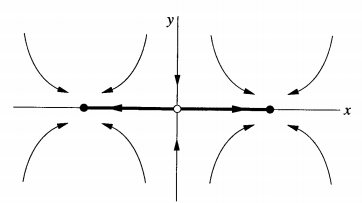
\includegraphics[width = 0.6\textwidth]{img/atractorExample.png}
\caption{Plano de fases asociado al sistema descrito en el ejemplo}
\label{fig:planoFasesAtractorEjemplo}
\end{figure}

Considerando el punto $(1,0)$ podemos observar que cumple las dos primeras propiedades de la definición de atractor. Sin embargo, no cumple la última propiedad, puesto que hay otro punto más que también satisface las propiedades necesarias.

Así, en este caso concreto, el atractor sería el conjunto
\[A=\{(\pm 1, 0)\}\]
\end{example}


Volviendo a los sistemas disipativos, estudiemos el caso del movimiento de un péndulo. La figura \ref{fig:pend_simple} muestra el comportamiento de un péndulo simple sobre el que no actúa la fuerza de la gravedad, mientras que la Figura \ref{fig:pend_amort} figura muestra el resultado de aplicarle dicha fuerza que amortigüa su movimiento haciéndolo cesar.

\begin{figure}[hbtp]
\centering
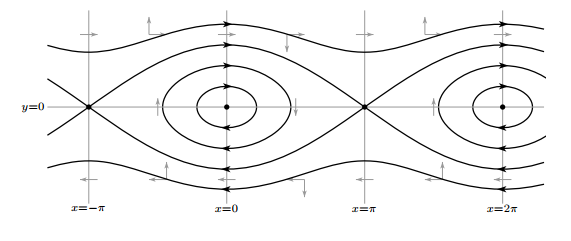
\includegraphics[width = 0.6\textwidth]{img/pend_simple.jpg}
\caption{Plano de fases del péndulo simple}
\label{fig:pend_simple}
\end{figure}

\begin{figure}[hbtp]
\centering
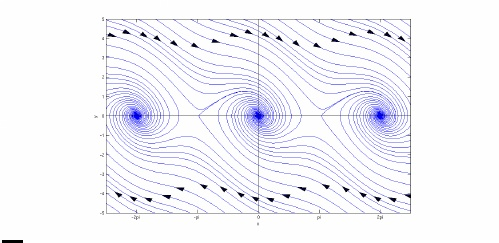
\includegraphics[width = 0.6\textwidth]{img/pend_amort.jpg}
\caption{Plano de fases del péndulo amortigüado}
\label{fig:pend_amort}
\end{figure}

En la Figura \ref{fig:pend_simple}, se puede observar que para posiciones angulares múltiplos pares de $\pi$, el sistema presenta puntos fijos (corresponde a mantener el péndulo en la posición vertical).

Nos interesa más la Figura \ref{fig:pend_amort}. En este caso, observamos que las posiciones que en el péndulo simple correspondían a puntos fijos, es decir, los múltiplos pares de $\pi$, ahora son \emph{atractores}. La velocidad angular del sistema decae a medida que la posición angular decrece por el \emph{efecto disipativo} del rozamiento.
\subsection{Flujos, compresibles o no}
La \textbf{compresibilidad} de un fluido es su propiedad para disminuir su volumen al aplicar presión o compresión. Todos los fluidos son compresibles en cierto grado. No obstante, los gases son altamente compresibles mientras que los líquidos son altamente incompresibles.

En condiciones regulares y a baja velocidad un fluido \emph{viscoso}, esto es, un fluido que presenta \emph{resistencia a fluir}, describe un \textbf{ movimiento estacionario}, es decir, las condiciones de velocidad en un punto dado no cambian con el tiempo. Cuando la velocidad del flujo es suficientemente grande, el movimiento se vuelve desordenado e irregular. En este caso hablamos de \textbf{flujo turbulento o caótico}. Un ejemplo de este caso es el ondear de una bandera al viento: si el flujo de aire fuera estacionario, la bandera ocuparía una posición fija a lo largo de las líneas de corriente, pero el asta rompe el flujo en un patrón irregular que da origen al movimiento de aleteo transversal de la bandera. En la Figura \ref{fig:flujo_turb} se observa un fluido con regiones de flujo estacionario (parte superior e inferior de la imagen) y regiones de flujo turbulento o caótico (zona central de la imagen).

\begin{figure}[hbtp]
\centering
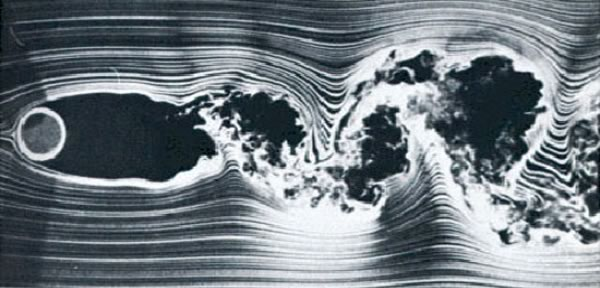
\includegraphics[width = 0.6\textwidth]{img/flujo_turb.jpg}
\caption{Flujo de un fluido}
\label{fig:flujo_turb}
\end{figure}


Podríamos pensar que el flujo turbulento de un cierto fluido es resultado de la ampliación de un movimiento que incluye tantas componentes de frecuencia que parece que se vuelve desordenado y confuso. Es decir, puede existir una estructura periódica subyacente, pero es demasiado compleja para seguirla.

La Teoría del Caos adquiere un enfoque diferente. El movimiento turbulento se debe a un comportamiento completamente \emph{aperiódico} y no simplemente una combinación de un gran número de movimientos periódicos. En este caso, el movimiento  deja de ser susceptible de predicción: 2 partículas que se muevan de forma parecida en el flujo en un tiempo dado pueden hallarse en estados de movimiento muy diferentes tras un lapso suficiente de tiempo.


\subsection{Atractores extraños: caos}

\begin{definition}[Atractor extraño]
A diferencia de los atractores que acabamos de ver, los atractores \textbf{extraños} tienen estructuras a todas las escalas. De modo que, un atractor es \emph{extraño} si tiene dimension de Hausdorff no entera o fractal o si la dinámica en el atractor es caótica.
\end{definition}
En los atractores extraños se observan órbitas irregulares, que las trayectorias divergen exponencialmente y que permanecen en un espacio de fases acotado.


Algunos de los ejemplos más importantes de atractores extraños son los siguientes:

\subsubsection{Mapa de Henón}
El mapa de Henón es un ejemplo de un sistema dinámico discreto en el tiempo y uno de los más estudiados cuando analizamos comportamientos caóticos. El mapa de Henón toma un punto en el plano $(x_n,y_n)$ y lo mapea en otro nuevo de la siguiente manera:\newline

$\left.
\begin{array}{rcl}
x_{n+1} & = & 1-ax^2_n+y_n\\
y_{n+1}& =& bx_n
\end{array}\right\}$\newline


El mapa depende de los parámetros a y b. Para el \textbf{mapa clásico de Henón} (Figura \ref{fig:henon_clas}) se cumple a=1.4 y b=0.3. En este caso, el mapa es \emph{caótico}. Para otros valores de a y b el mapa puede ser caótico, intermitente o converger a una órbita periódica.

\begin{figure}[hbtp]
\centering
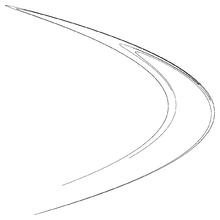
\includegraphics[width = 0.3\textwidth]{img/henon_clas.png}
\caption{Atractor de Henón para a=1.4 y b=0.3}
\label{fig:henon_clas}
\end{figure}

La Figura \ref{fig:henon_orb} muestra el diagrama de órbitas del mapa de Henón para b=0.3. En el diagrama se muestran los valores de la variable $x$ en función del parámetro a. Para valores de a próximos a 1 el período de oscilación es 8 y a partir de a=1.04 aproximadamente, se produce el llamado \emph{period doubling-cascade}, es decir,  el período de oscilación se dobla a 16 y así sucesivamente. A partir de a=1.08 la naturaleza del atractor cambia drásticamente de su condición de periodicidad a caótica. Aún así es posible observar zonas de periocidad intercaladas en aquellas caóticas, como es el caso de los puntos próximas a a=1.25 dónde encontramos órbitas de período 6.

\begin{figure}[hbtp]
\centering
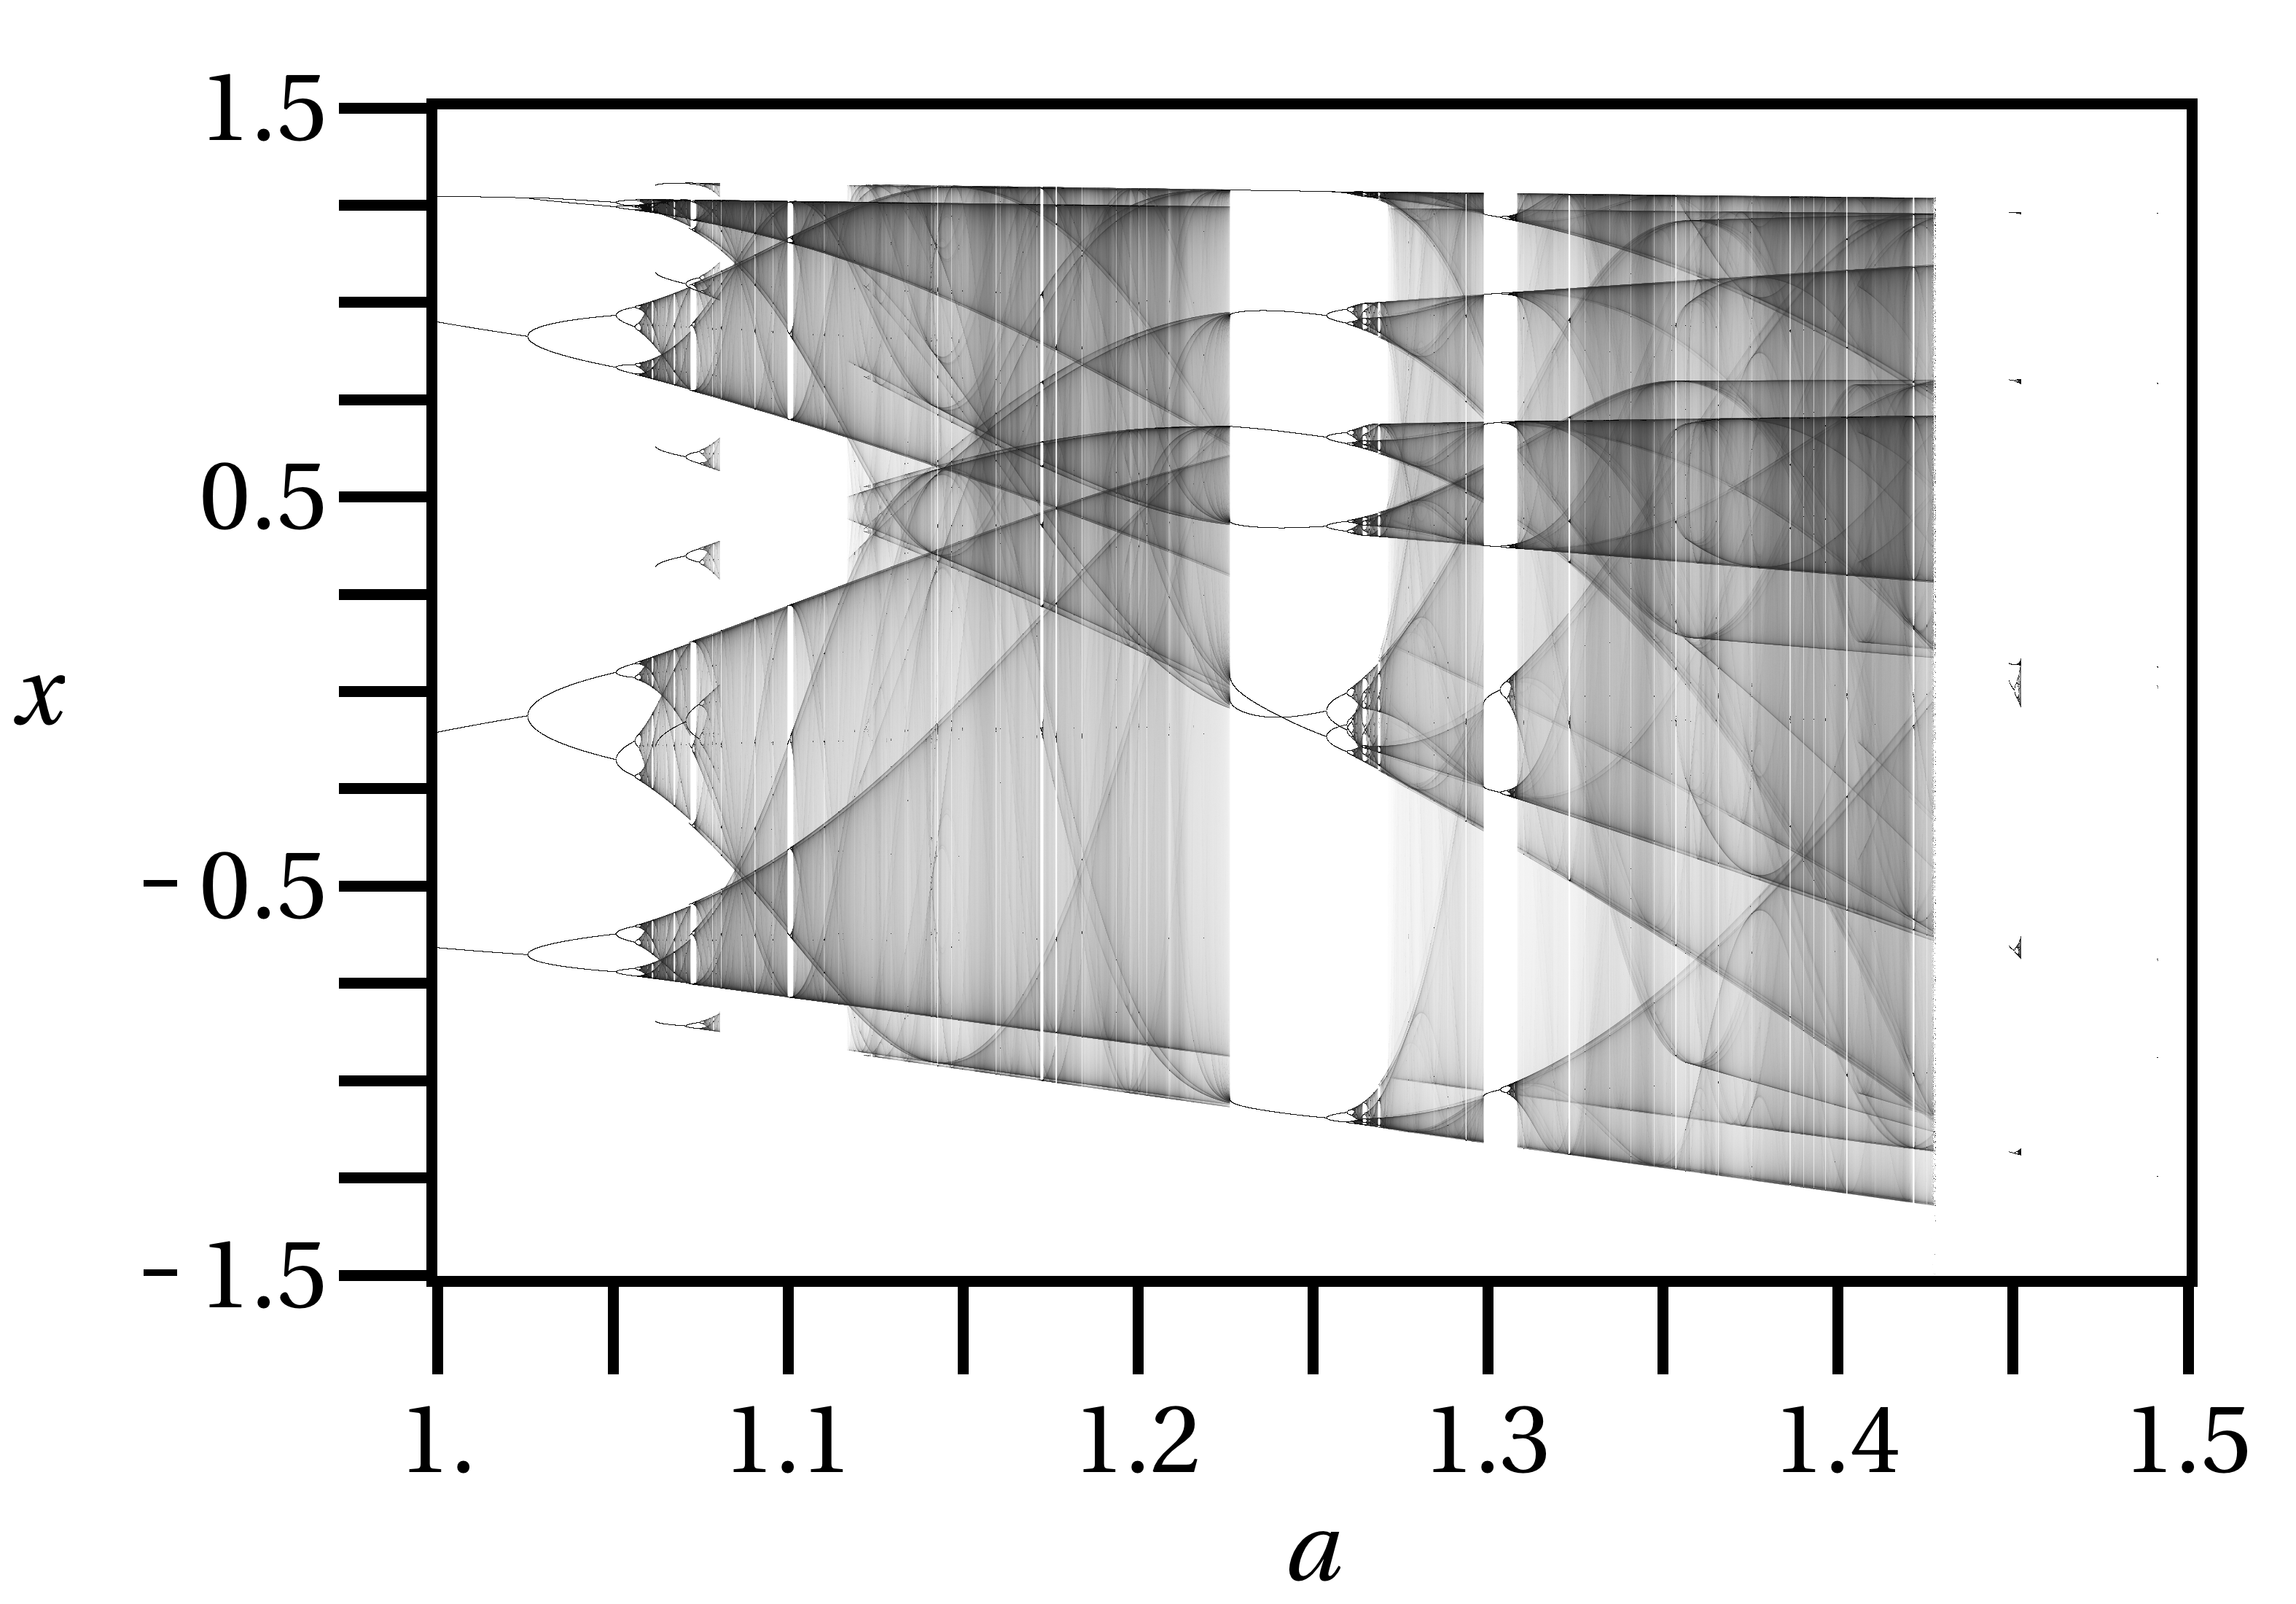
\includegraphics[width = 0.6\textwidth]{img/henon_orb.png}
\caption{Esquema de órbita para el mapa de Henón con b=0.3}
\label{fig:henon_orb}
\end{figure}

%\subsubsection{Atractor de Rössler}
%Este atractor aparece en el \emph{sistema de Rössler}, un sistema de ecuaciones diferenciales que definen un sistema dinámico continuo que muestra trayectorias caóticas asociadas con las propiedades fractales del atractor.
%
%\begin{figure}[hbtp]
%\centering
%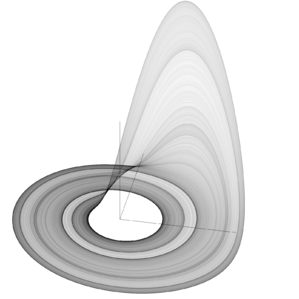
\includegraphics[width = 0.4\textwidth]{img/rossler.png}
%\caption{Atractor de Rössler}
%\label{fig:rossler}
%\end{figure}


\subsubsection{Atractor de Lorenz}
Este atractor, introducido por Edward Lorenz en 1963, es un sistema dinámico determinista tridimensional no lineal que deriva de las ecuaciones simplicadas de rollos de convección (estos son formas de transferencia de calor en un fluido, por ejemplo, el aire de la atmósfera) que se producen en la atmósfera de nuestro planeta.

Tanto las ecuaciones como la representación de estos atractores se detallan en la siguiente sección.

\subsection{Ecuaciones de Lorenz}
\begin{definition}[Ecuaciones de Lorenz]
En 1963 Lorenz desarrolló un sistema de ecuaciones tridimensional que modelizaba, de manera extraordinariamente simple, la convección en forma de anillos que parece ocurrir a veces en la atmósfera terrestre.

El sistema descrito por Lorenz fue:
\[\begin{array}{l}
x'(t) = σ(y(t)-x(t)) \\
y'(t) = rx(t)-y(t)-x(t)y(t)\\
z'(t) = x(t)y(t)-bz(t)
\end{array}\]
donde σ es el \textbf{número de Prandtl}, que representa la viscosidad/conductividad térmica, $r$ es el \textbf{número de Rayleigh}, que representa la diferencia de temperatura entre base y tope y $b$ es la razón entre la longitud y altura del sistema.
\end{definition}

Lorenz descubrió que este sistema de apariencia tan sencilla escondía un comportamiento realmente caótico. Las soluciones oscilaban de manera irregular, sin repetirse nunca el mismo patrón pero manteniéndose siempre dentro de una región limitada del plano de fases. Como puede verse en la figura \ref{fig:Lorenz} la solución de las ecuaciones da lugar a un complicado conjunto \emph{con forma de mariposa} conocido hoy en día como \textbf{atractor extraño}. A diferencia de los puntos fijos estables, el \textbf{atractor extraño} no es un punto ni una curva ni si quiera una superficie, es un \emph{fractal} con dimensión fractal entre 2 y 3.

\begin{figure}[hbtp]
\centering
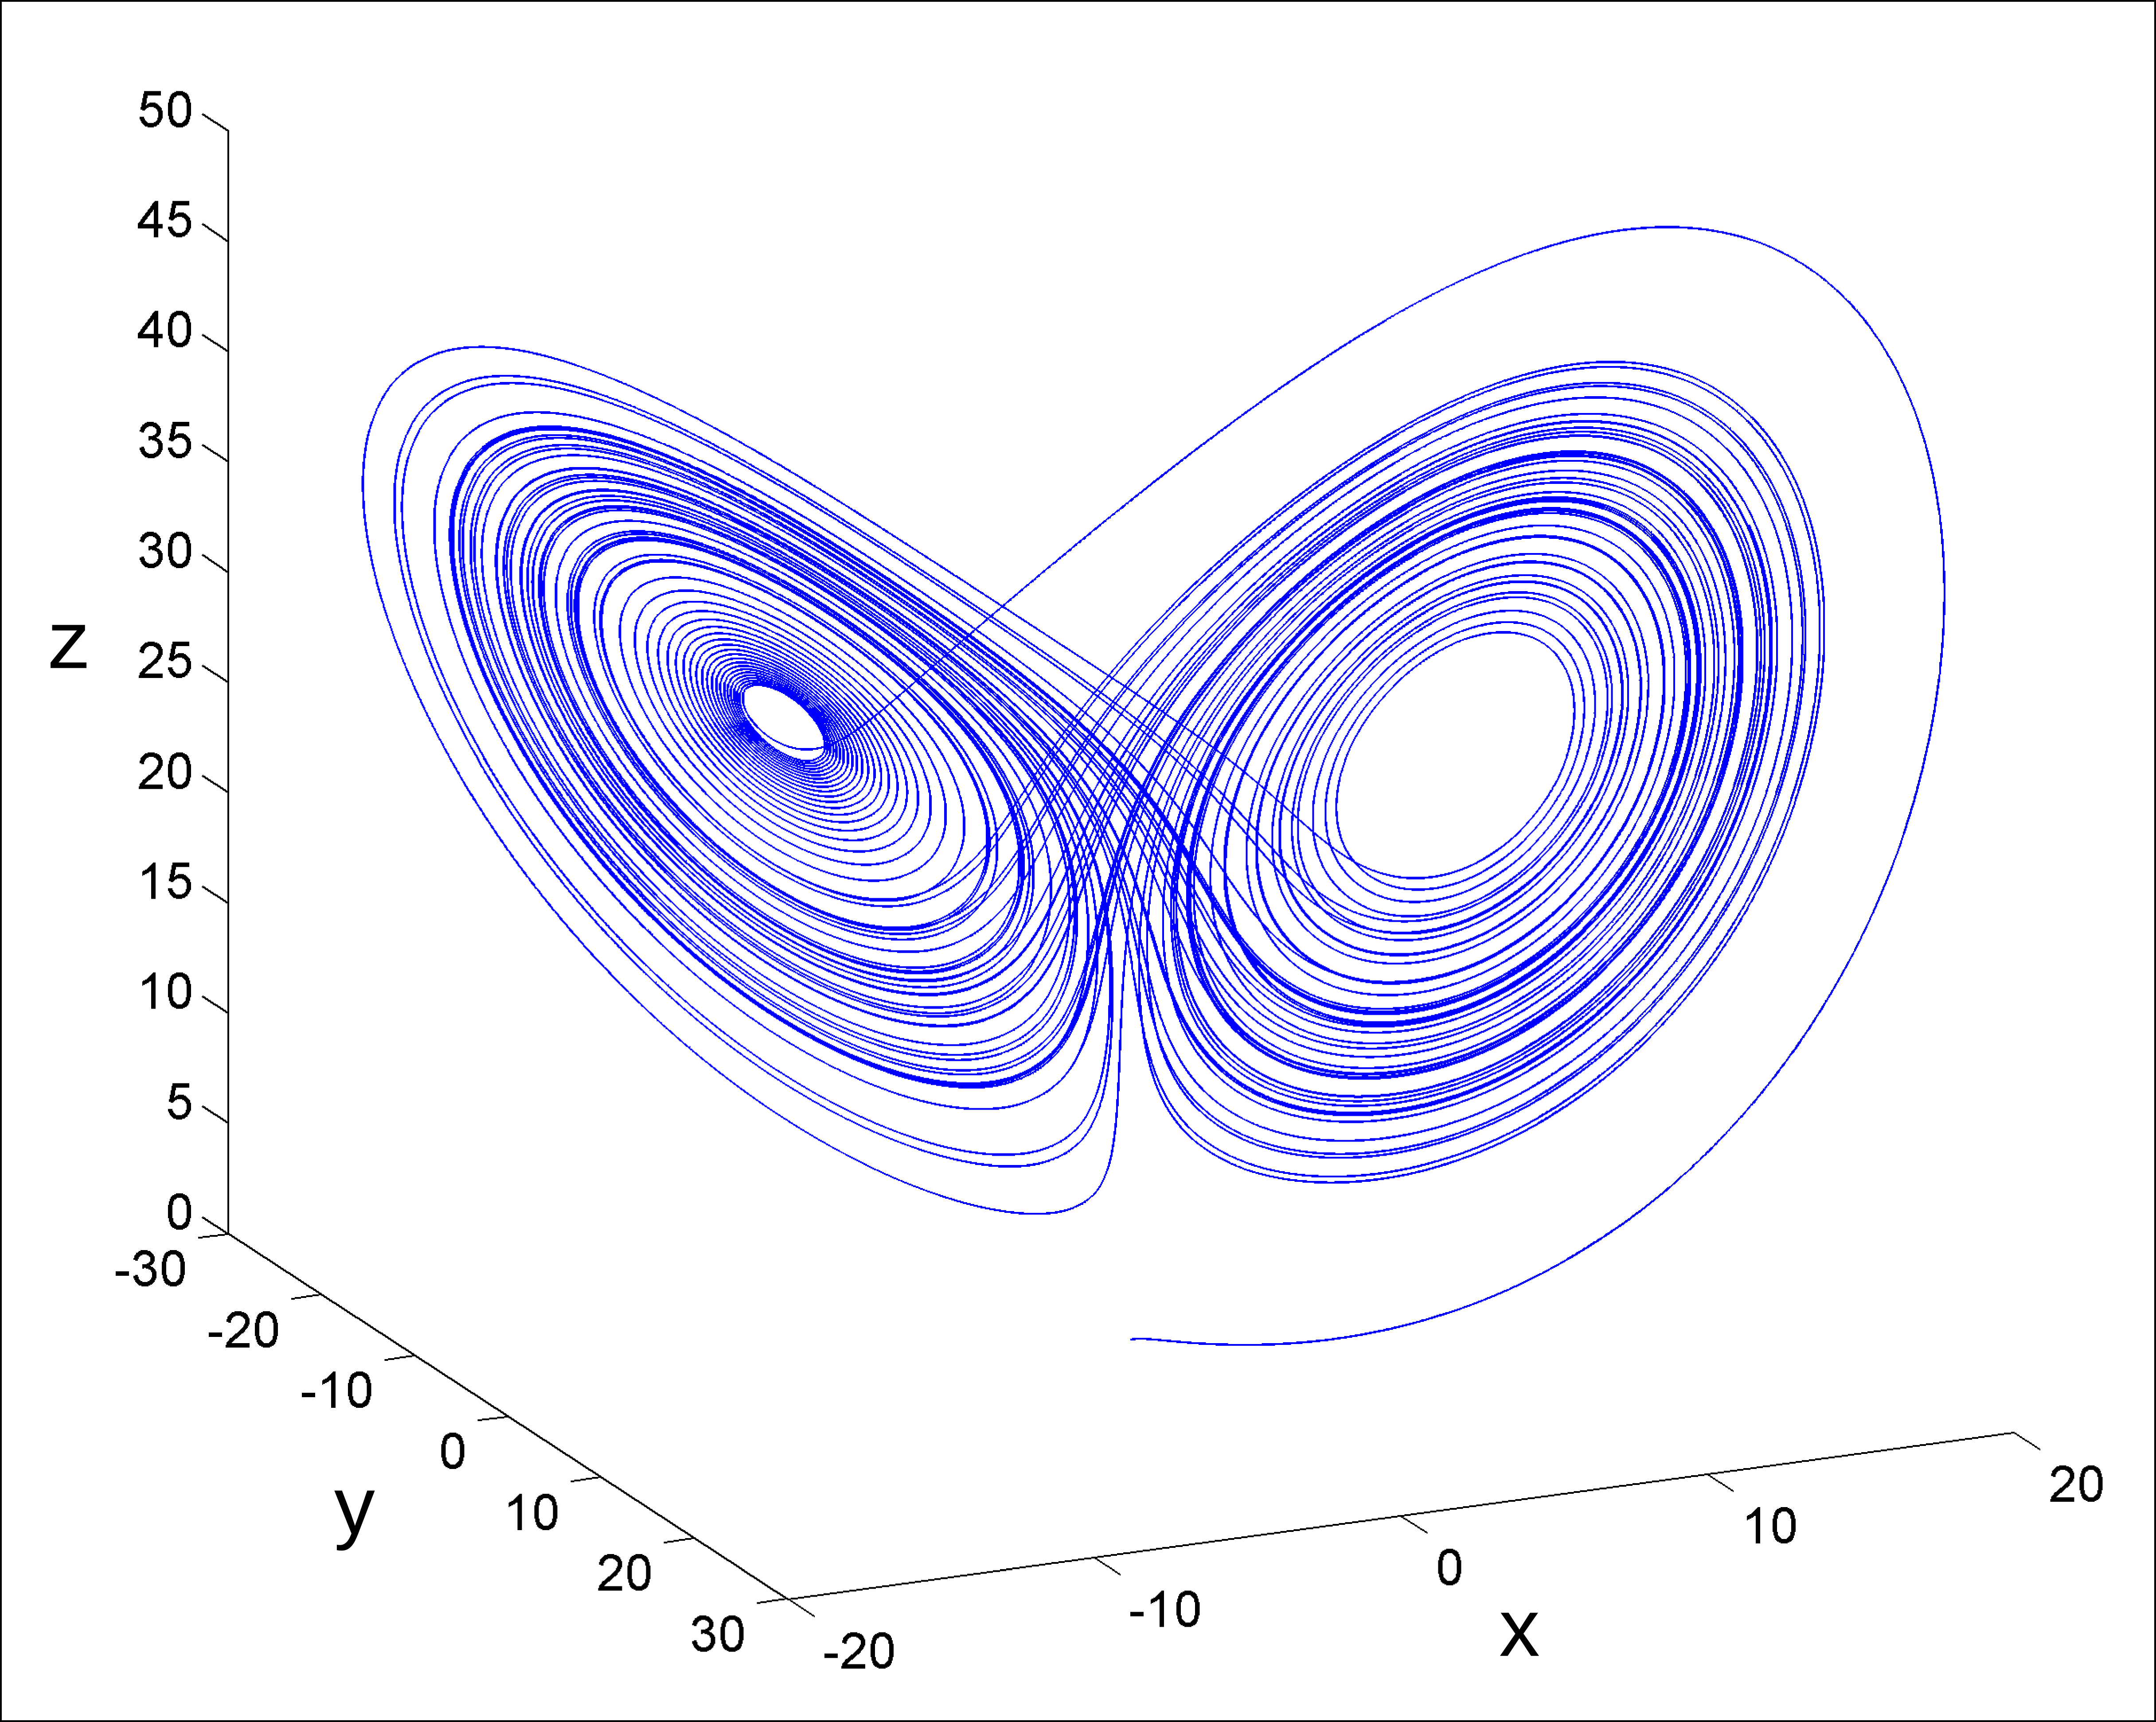
\includegraphics[width = 0.6\textwidth]{img/Lorenz.png}
\caption{Representación tridimensional de la solución de las ecuaciones de Lorenz}
\label{fig:Lorenz}
\end{figure}

\subsubsection{Algunas propiedades de las ecuaciones de Lorenz}
Lorenz publicó un artículo donde llevaba a cabo un análisis muy detallado de sus ecuaciones. Llevó el análisis tan lejos como pudo empleando ténicas estandarizadas pero, una vez llegado a cierto punto, se topó con lo que parecía un \emph{paradoja}. Una a una fue eliminando todas las posibilidades acerca del comportamiento del sistema a largo plazo.

Probó que, dentro de un cierto rango de parámetros, el sistema no tendría puntos fijos estables ni ciclos finitos estables. No obstante, también demostró que las soluciones no salían de una cierta región \emph{delimitada} y que, llegado a cierto punto, se veían atraídas hacia un conjunto de volumen cero. Este conjunto es lo que se conoce como \textbf{atractor extraño}.

Veamos por encima las propiedades del sistema que Lorenz estudió en su famoso artículo.

\begin{itemize}
\item \textbf{No linearidad}
El sistema de Lorenz presenta dos términos no lineales: $x(t)y(t)$ y $x(t)z(t)$.

\item \textbf{Simetría}
Si reemplazamos los términos $x(t)$ e $y(t)$ por $-x(t)$ y $-y(t)$ respectivamente obtenemos un sistema equivalente:
\[\begin{array}{l}
-x'(t) = -σ(y(t)-x(t)) \\
-y'(t) = -rx(t)+y(t)-x(t)y(t)\\
z'(t) = x(t)y(t)-bz(t)
\end{array}\]

Es decir, si $(x(t),y(t),z(t))$ es una solución también lo será $(-x(t),-y(t),z(t))$.

\item \textbf{Contracción de volumen}
El sistema de Lorenz es \emph{disipativo}: el volumen en el plano de fases se contrae. Para comprender esto lo primero que debemos hacer es ver cómo evoluciona este volumen.

Para cualquier sistema tridimensional $\vec{x}'(t) =f(\vec{x}(t))$, consideramos una superficie cerrada $S(t)$ de volumen $V(t)$ en el plano de fases. Consideremos ahora los puntos de $S(t)$ como puntos iniciales para diferentes trayectorias y veamos su evolución durante un instante de tiempo infinitesimal $dt$. Tras este tiempo $S(t)$ se convierte en una nueva superficie $S(t+dt)$.

La figura \ref{fig:volumen2D} representa en dos dimensiones la situación recien descrita.
\begin{figure}[hbtp]
\centering
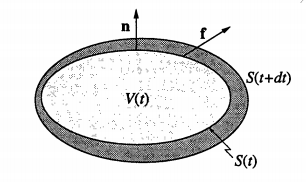
\includegraphics[width = 0.6\textwidth]{img/volumen2D.png}
\caption{Evolución con el tiempo de la superficie y del volumen contenido en su interior, siendo \textbf{n} el vector normal a la superfice $S(t)$}
\label{fig:volumen2D}
\end{figure}

El volumen encerrado por la nueva superficie cerrada puede escribirse como
\[V(t+dt)=V(t) + \int_S (f\cdot \text{\textbf{n}}\ dt)\ dA\]

Puesto que
\[V'(t)=\frac{V(t+dt)-V(t)}{dt} = \int_S f\cdot \text{\textbf{n}}\ dA\]

Aplicando el teorema de divergencia podemos reescribir la integral como:
\[V'(t) = \int_V \nabla \cdot f \ dV \]
siendo, para el sistema de Lorenz
\[\nabla \cdot f = \frac{\partial}{\partial x}[σ(x-y)] + \frac{\partial}{\partial y}[rx-y-xy] + \frac{\partial}{\partial z}[xy-bz] = -σ-1-b < 0\]

Puesto que la divergencia es constante, la ecuación de la derivada del volumen queda
\[V'(t) = -(σ+1+b)V(t) \implies V(t) = V(0)e^{-(σ+1+b)t}\]
con lo que queda claro que el volumen de crece de manera exponencial.

\item \textbf{Puntos fijos}
El sistema de Lorenz tiene ``dos tipos de puntos fijos''.

Por un lado tenemos el punto fijo $(0,0,0)$ que lo es para cualquier combinación de parámetros que decidamos tomar. Por otro, tenemos puntos fijos que dependen de los parámetros seleccionados. Así
\[(\pm \sqrt{b(r-1)},\pm \sqrt{b(r-1)},r-1) \text{ para } r>1\]
es un punto fijo del sistema.

Lorenz definió como $C^+$ el conjunto de puntos fijos como el descrito anteriormente tomando el signo positivo donde hay dos posibilidades. Simétricamente, definió el conjunto $C^-$.

\item \textbf{Estabilidad lineal del origen}

Omitiendo las dos \emph{no linearidades} del sistema de Lorenz obtenemos una linearización del sistema en torno al origen
\[\begin{array}{l}
x'(t) = σ(y(t)-x(t)) \\
y'(t) = rx(t)-y(t)\\
z'(t) = -bz(t)
\end{array}\]

La ecuación para la $z(t)$ es independiente de las otras dos y muestra, de manera trivial, un crecimiento exponencial de $z(t)$. Las otras dos ecuaciones del sistema pueden escribirse como una ecuación matricial de la forma:

\[\left(\begin{array}{l}
x'(t) \\ y'(t)
\end{array} \right)\left(\begin{array}{cc}
-σ & σ \\ r & -1
\end{array} \right)\left(\begin{array}{l}
x(t) \\ y(t)
\end{array} \right)\]

La traza de la matriz es $τ=-σ-1<0$ y el determinante $Δ = σ(1-r)$. Si $r>1$ el origen es un \emph{punto de silla} pueso que $Δ<0$. Por otro lado, si $r<1$ entonces nos encontramos ante un sumidero, pues todas las direcciones convergen hacia el origen. En concreto, el origen es un nodo estable para $r<1$.

\item \textbf{Estabilidad global del origen}

Puede comprobarse que para $r<1$ toda trayectoria tiende al origen a medida que $t$ tiende a infinito. Por tanto el origen es \emph{globalmente estable}. Por tanto, no puede haber ciclos infinitos ni caos para $r<1$.

\end{itemize}

\subsection{Órbitas caóticas y exponentes de Lyapunov}

El concepto de equilibrio inestable es muy común en física, y en general, en cualquier ciencia. A pesar de que, en teoría podemos colocar una pelota en el pico de una montaña de manera que permanezca en un estado de equilibrio y no se mueva, en la práctica es imposible: el estado de equilibrio estático es \emph{inestable}. La trayectoria de cualquier posición inicial le hará salir de ese estado de equilibrio, posiblemente para pasar a otro, tal vez pasar a colocarse en un valle a una altura menor. Un tipo de comportamiento muy común en algunos sistemas dinámicos es pasar de una posición inicial en un estado de equilibrio inestable atraídos por un estado de equilibrio \emph{estático} \emph{estable} o un estado \emph{periódico estable}.

Pero esto no siempre ocurre. De hecho esta es una de las características más importantes de estados las \textbf{órbitas caóticas}. Éstas son aquellas que permanecen infinitamente en un estado inestable, sin llegar a ser converger o ser atraídas hacia níngun estado estático o periódico estable. Esta irregularidad es cuantificada mediante los \textbf{números de Lyapunov} y los \textbf{exponentes de Lyapunov}.

Informalmente, diremos que el \textbf{número de Lyapunov} es la tasa o razón media a la que los puntos divergen a lo largo de la órbita. Diremos que el \textbf{exponente de Lyapunov} es el logaritmo natural del número de Lyapunov.

Encontramos \emph{caos} cuando los coeficientes de Lyapunov de nuestro sistema dinámico son mayores que 1.

A continuación definimos formalmente el concepto de exponente  de Lyapunov:

\begin{definition}[Exponente de Lyapunov]
Dado un dato inicial $x_0$ consideramos un dato cercano $x_0+ε_0$, como ya hicimos en el ejemplo \ref{example:Julia} siendo la separación $ε_0$ extremadamente pequeña.

Sea $ε_n$ la separación tras $n$ iteraciones, si se da la relación $|ε_n|\approx e^{n\cdot λ}|ε_0|$, decimos que λ es el \textbf{exponente de Lyapunov}.
\end{definition}

\begin{example}
Vamos a calcular el exponente de Lyapunov para el caso concreto
\[f(x) = \left\{ \begin{array}{ll}
rx, & 0 \leq x \leq \frac{1}{2}\\
r-rx, & \frac{1}{2} < x \leq 1
\end{array}\right.\]

De forma genérica tendremos:
\[ε_n = f^n(x_0+ε_0)-f^n(x_0) \]
y queremos escribir
\[|ε_n| = |ε_0| e^{nλ} \implies λ = \frac{1}{n} \ln\left| \frac{ε_n}{ε_0}\right| = \frac{1}{n}\ln \left|\frac{f^n(x_0+ε_0)-f^n(x_0)}{ε_0} \right| = \frac{1}{n}\ln \left|(f^n)'(x_0) \right|\]
donde en el último paso hemos considerado $ε_0 \to 0$.

Aplicando la regla de la cadena podemos escribir
\[(f^n)'(x_0) = \prod_{i=0}^{n-1}f'(x_i) \]

Razonando sobre los multiplicadores podemos escribir
\[\ln \left|\prod_{i=0}^{n-1}f'(x_i)\right| = \sum{i=0}^{n-1}\ln |f'(x_i)| \]

En esta ocasión tenemos $f'(x)=\pm r$ para todo $x$ lo que nos lleva a
\[λ= \frac{1}{n}\sum_{i=0}^{n-1}\ln |f'(x_i)| = \ln r\]
\end{example}

Cabe remarcar que por tratarse de un problema 1-dimensional, sólo hemos obtenido 1 exponente de Lyapunov. Si el problema hubiera sido 2-dimensional hubiéramos calculado 2 y así sucesivamente.

Aquellas órbitas que convergen a orbitas periódicas comparten los mismos exponentes de Lyapunov. Pero, más interesante es el caso de órbitas que no convergen asintóticamente (a largo plazo) a órbitas periódicas. Cuando estamos en ese caso y la órbita presenta coeficientes de Lyapunov \emph{positivos}, diremos que la órbita es \textbf{caótica}.

\begin{definition}(Órbita caótica)
Una órbita es caótica si:
\begin{itemize}
\item No es asintóticamente periódica.
\item Sus exponentes de Lyapunov son mayores que cero.
\end{itemize}
\end{definition}

% \subsection{Ejemplos de sistemas}
% Para los ejemplos: Non linear dynamic and chaos.
% Creo que esto sobra. Los ejemplos ya los hemos ido incluyendo cuando lo hemos considerado necesario.


%%%%%%%%%%%%%%%%%%%%%%%%%%%%%%%%%%%%%%%%%%%%%%%%%%%%%%%%%%
%%%%%%%%%%%%%%%%%%%%%%%%%%%%%%%%%%%%%%%%%%%%%%%%%%%%%%%%%%
%%%%%%%%%%%%%%%%%%%%%%%%%%%%%%%%%%%%%%%%%%%%%%%%%%%%%%%%%%
%%%%%%%%%%%%%%%%%%%%%%%%%%%%%%%%%%%%%%%%%%%%%%%%%%%%%%%%%%
%%%%%%%%%%%%%%%%%%%%%%%%%%%%%%%%%%%%%%%%%%%%%%%%%%%%%%%%%%
%%%%%%%%%%%%%%%%%%%%%%%%%%%%%%%%%%%%%%%%%%%%%%%%%%%%%%%%%%
%%%%%%%%%%%%%%%%%%%%%%%%%%%%%%%%%%%%%%%%%%%%%%%%%%%%%%%%%%
%%%%%%%%%%%%%%%%%%%%%%%%%%%%%%%%%%%%%%%%%%%%%%%%%%%%%%%%%%
%%%%%%%%%%%%%%%%%%%%%%%%%%%%%%%%%%%%%%%%%%%%%%%%%%%%%%%%%%

\lstset{language=Matlab,%
    %basicstyle=\color{red},
    breaklines=true,%
    morekeywords={matlab2tikz},
    keywordstyle=\color{blue},%
    morekeywords=[2]{1}, keywordstyle=[2]{\color{black}},
    identifierstyle=\color{black},%
    stringstyle=\color{mylilas},
    commentstyle=\color{mygreen},%
    showstringspaces=false,%without this there will be a symbol in the places where there is a space
    numbers=left,%
    numberstyle={\tiny \color{black}},% size of the numbers
    numbersep=9pt, % this defines how far the numbers are from the text
    emph=[1]{for,end,break},emphstyle=[1]\color{red}, %some words to emphasise
    %emph=[2]{word1,word2}, emphstyle=[2]{style},
}

\section{Aplicaciones}
\subsection{Generación gráfica de conjuntos de Julia}
Los siguientes dos ficheros permiten generar, en Octave, conjuntos de Julia creados sobre la ecuación $z=z^2+c$ siendo el valor de la constante elegido libremente por el usuario.

\lstinputlisting{mjcore.m}
\lstinputlisting{Julia.m}

Ejecutando el código tal cual se muestra en estos fragmente obtenemos la figura \ref{fig:JuliaOctave}

\begin{figure}[hbtp]
\centering
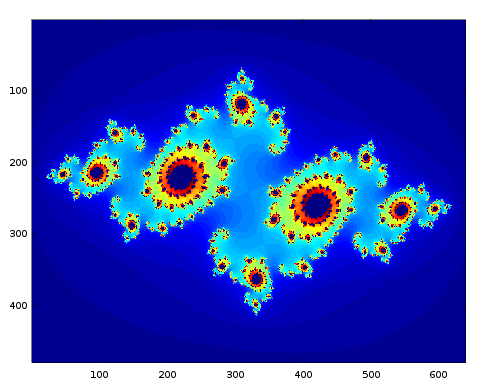
\includegraphics[width = 0.6\textwidth]{img/JuliaOctave.png}
\caption{Conjunto de Julia obtenido mediante Octave}
\label{fig:JuliaOctave}
\end{figure}

\subsection{Ejemplos gráficos de explorar el conjunto de Mandelbrot}
El siguiente fragmento de código permite dibujar conjuntos de Mandelbrot con Octave

\lstinputlisting{mandelbrot.m}

Ejecutando el fragmento de código tal cual se muestra obtenemos la imagen representada en la figura \ref{fig:MandelbrotOctave}
\begin{figure}[hbtp]
\centering
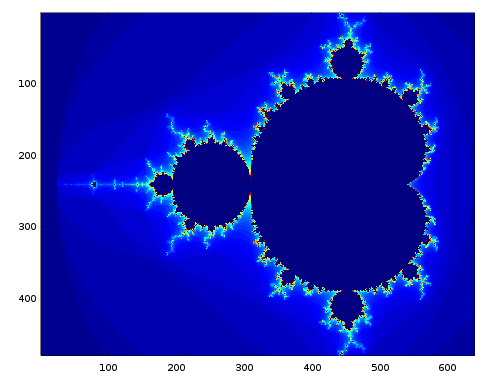
\includegraphics[width = 0.6\textwidth]{img/mandelbrotOctave.png}
\caption{Conjunto de Mandelbrot obtenido mediante Octave}
\label{fig:MandelbrotOctave}
\end{figure}

\subsection{Caos y criptografía}
La ciencia de la criptografía se ocupa de los problemas de la seguridad de la información y sus pertinentes almacenamientos y transferencias.

Los fractales y los sistemas caóticos tienen características que se han estudiado extensivamente a través de los años, y su complejidad inherente deriva de la sensibilidad extrema del sistema a las condiciones iniciales. Muchos de los sistemas caóticos tienen la característica de que no existe ninguna solución de forma cerrada para ellos, y por lo tanto no existen las fórmulas ``simples" que definan al sistema en cualquier punto dado. En relación a la criptografía, esto califica como problema muy difícil de resolver. La principal ventaja de los sistemas caóticos, es que son probabilisticamente difíciles, eliminando una de las desventajas fundamentales de la criptografía convencional.

\begin{definition}[Criptografía fractal]
La criptografía fractal o caótica aplica fractales y sistemas caóticos para obtener métodos criptográficos.
\end{definition}

\subsubsection{Usando una función caótica pare encriptar}
La seguridad de este tipo de criptosistema se basa en la esperanza de que sin conocer la clave secreta, el comportamiento caótico sea lo suficientemente difícil de predecir utilizando métodos analíticos. Esto reduciría los posibles ataques a una sola categoría, los ataques de fuerza bruta, en los cuales se prueban todas las claves posibles contra los datos encriptados. Los ataques de fuerza bruta rara vez son exitosos ya que dependen directamente de la longitud de la clave utilizada.

Veamos un ejemplo de cifrado criptográfico.

\begin{example}[Cifrado por bloques simple]
Este es un algoritmo de cifrado por bloques con una clave secreta. La clave es utilizada para generar un pad que luego es combinado con el texto en claro por bloques de 8 bits.

En este cifrador, las claves de sesión forman parte de la clave de encriptación y se toman en forma cíclica. Por ejemplo si se utiliza una clave de 256 bits, las claves de sesión irán desde la $k_1$ a la $k_{256}$.

\begin{figure}[H]
\centering
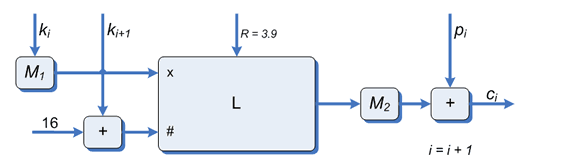
\includegraphics[width = \textwidth]{img/cifradoCaotico.png}
\end{figure}

El modo en que se genera el pad consiste en tomar dos claves de sesión sucesivas $k_i$ y $k_{i+1}$ y en lugar de combinarlas directamente con el texto en claro, se utilizan como condiciones iniciales para el mapa caótico.

El bloque $M_1$ representa un mapeo del espacio de claves de sesión, todos los enteros entre el 0 y 255, en el dominio del mapa logístico $L$, todos los reales en el intervalo [0,1]. La suma de la siguiente clave de sesión y el número 16 es usada como el número de iteraciones del mapa logistico. $M_2$ usa un subconjunto difuso\footnote{Un subconjunto difuso, es un conjunto que puede contener elementos de forma parcial, es decir que la propiedad  $x\in A$ puede ser cierta, falsa o solamente posible.} para mapear el dominio del mapa logístico, reales entre 0 y 1, nuevamente al intervalo discreto [0,255]. A medida que se encripta un nuevo bloque, el contador $i$ usado para llevar un registro de la clave de sesión actual es incrementado. La salida del mapa logístico es combinada con el texto en claro para dar el texto encriptado.

El proceso de desencriptado es simple, el mismo pad es generado a partir de la clave y se utiliza para descombinarlo del texto encriptado para recuperar el texto en claro.

En un análisis sencillo de este cifrador se ve que posee buenas propiedades estadísticas. Sin embargo por más que estadísticamente luce bien, haciendo una comparación gráfica tomando como texto claro una imagen y comparándo la imagen sin encriptar con su contraparte encriptada se puede observar que gran cantidad de la información de la imagen original es visible en la imagen cifrada. Este problema ocurre por que el pad producido por el cifrador depende solo de la clave y por lo tanto pose un periodo del tamaño de la clave. Esto significa que series del mismo pad son utilizadas en forma repetida dando lugar a patrones de posicionamiento. Los patrones son fácilmente reconocidos por el ojo humano y aunque los colores hayan cambiado, aun es posible distinguir de qué se trata la imagen original, como muestran las figuras \ref{fig:ImagenCifrada}

\begin{figure}[hbpt]
\centering
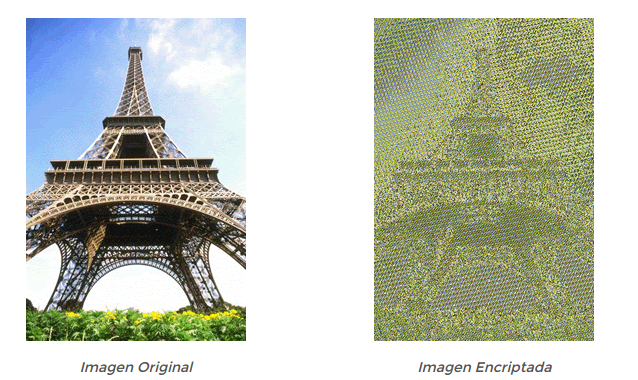
\includegraphics[width = 0.8\textwidth]{img/imagenCifrada.png}
\caption{Comparación de imagen original con su versión cifrada}
\label{fig:ImagenCifrada}
\end{figure}

El comportamiento periódico del cifrador es un indicio de que el mismo no es seguro. Un método que se puede utilizar para resolver este problema es agregando retroalimentación al mecanismo del cifrador. De esta forma la encriptación no solo dependerá de la clave sino que también dependerá del texto en claro encriptado previamente.

\begin{figure}[H]
\centering
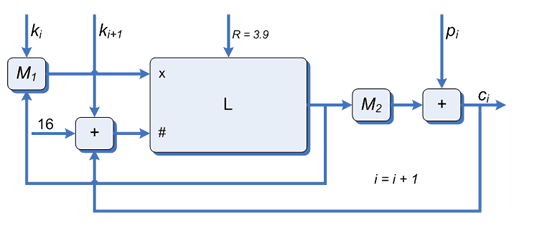
\includegraphics[width = \textwidth]{img/cifradoCaoticoRetro.png}
\end{figure}

Por ejemplo una forma de retroalimentación es utilizar la salida de la función caótica ya añadirla a la entrada para obtener el nuevo x. Además el valor numérico del bloque anterior es añadido al número de iteraciones.

Estas modificaciones hacen que el cifrador funcione mucho mejor que antes y que el fantasma de la imagen original que podía apreciarse en la imagen encriptada prácticamente desaparezca, como muestran las figuras \ref{fig:ImagenCifradaRetro}

\begin{figure}[hbpt]
\centering
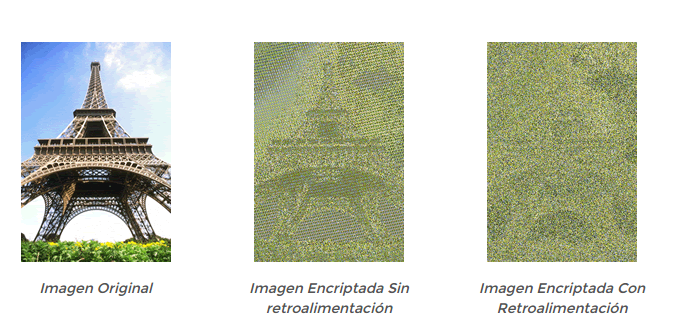
\includegraphics[width = \textwidth]{img/imagenCifradaRetro.png}
\caption{Comparación de imagen original con su versión cifrada y su versión con el cifrado mejorado}
\label{fig:ImagenCifradaRetro}
\end{figure}

\subsection{Compresión fractal}\label{sec:compresionFractal}
La compresión fractal es una tecnología bastante controvertida, con detractores y admiradores. La idea básica detrás de la compresión fractal de imágenes, es expresar la imagen como un sistema de funciones iteradas (IFS). La imagen puede mostrarse rápidamente, y un zoom proporciona infinitos niveles de detalles fractales (sintéticos).

El problema es cómo generar eficientemente la imagen IFS.

Hay cuatro características de la tecnología IFS que es necesario conocer para entender su situación actual:
\begin{itemize}
\item Es un método de compresión que pierde un poco de información (como JPG).
\item La resolución al agrandar es poderosa, pero no una forma de comprimir 100:1.
\item La compresión es lenta, la descompresión es rápida.
\item La tecnología está patentada.
\end{itemize}

Dado que los fractales matemáticos servían para generar imágenes que se veían naturales, se pensó que también podría servir en el sentido opuesto: para comprimirlas.

La idea es tomar una imagen y llevarla a un sistema de funciones iterado, que podría generar el original. No obstante este problema aun no se ha resuelto.

Fue Barnsley, quien en 1988 anunció al mundo que \textbf{si} lo había resuelto, patentando la tecnología. El problema fue que tomaba alrededor de 100 horas para codificar una imagen, y alrededor de 30 minutos para decodificarla, con una persona guiando el proceso. El resultado era una compresión 10.000:1. Poco después con uno de sus alumnos de doctorado, desarrolló un sistema para representar imágenes llamado \textbf{Sistema de Funciones Iteradas Particionado (PIFS)}. Se trataba de un algoritmo que comprimía automáticamente la imagen en un \emph{Sistema de Funciones Iterado Particionado}. El algoritmo no era sofisticado, ni rápido, pero si automático. El costo fue que una imagen codificado con colores de 24-bit podía ser comprimida de 8:1 a 50:1, lo cual aún es bastante bueno.

Todos los programas actuales de compresión de imágenes fractales (que no son muchos) se basan es este algoritmo. La empresa ``Iterated Systems", vende el único compresor/decompresor comercial, llamado ``Images Incorporated". También hay varios programas de académicos disponibles gratuitamente en Internet.

Actualmente la técnica de compresión fractal no supera el estándar de compresión de imágenes JPEG ni el JPEG2000.

\subsection{Antenas fractales}

En la pasada década, los científicos han comenzado a aplicar los fractales a un tema algo \emph{oscuro}: el diseño de las antenas.

Las antenas parecen ser simples, pero la teoría que tienen detrás, basadas en las ecuaciones de Maxwell del electromagnetismo, son impenetrables. Como resultado, los ingenieros de antenas tienen que usar el método de prueba y error. Incluso los mejores y más tecnológicos receptores dependen habitualmente de un hilo que no es mejor que el que usó Marconi para la radio hace cien años.

Los fractales ayudan de dos formas. Primero, pueden mejorar el funcionamiento de los conjuntos de antenas. Muchas antenas parecen estar compuestas de una unidad independiente, incluyendo la mayoría de antenas de radar, pero en realidad están compuestas de formaciones de cientos de pequeñas antenas. Tradicionalmente, estas antenas individuales se colocan de forma aleatoria o de forma ordenada pero Dwight Jaggard, de la Universidad de Pensilvana, junto con otras personas, han descubierto que una colocación en forma de fractal puede combinar la robustez de una colocación aleatoria con la eficiencia de una ordenación coherente, con una reducción significativa del número de elementos necesarios.

``Los fractales son el puente que llena los hueco", comenta Jaggard, ``tienen un desorden a corto alcance y un orden a largo alcance". Incluso las antenas independientes se benefician de tener una forma fractal. Nathan Cohen, un radio astrónomo de la Universidad de Boston, ha experimentado con los cables fractales, conocidos como curvas Koch o triángulos de Sierpinski. No sólo se puede meter la misma longitud de antena en una sexta parte del área, sino que las formas angulares generan capacidades eléctricas y conductividad, eliminando el inconveniente de que los componentes externos sintonicen la antena entre el rango de frecuencias a las que responden.

El por qué las antenas fractales funcionen tan bien fue probado matemáticamente por Cohen y Robert Hohlfeld, quienes establecieron que una buena antena fractal debe satisfacer dos condiciones
\begin{enumerate}
\item Tiene que ser simétrica con respecto a un punto
\item Tiene que ser similar a sí misma (es decir, tener el mismo aspecto básico en cada escala), para poder ser fractal.
\end{enumerate}

Posiblemente, en un futuro cercano, estas antenas fractales tendrán un uso masivo en el nuevo \textbf{Sistema de Identificación por Radiofrecuencia} que sustituirá a los códigos de barras habituales.
\end{example}

\subsection{Teoría del Caos y Aeronaútica}
Tener ciertas condiciones de \textbf{estabilidad} es muy conveniente en numerosos escenarios y más cuando se trata de manetener aviones suspendidos en el aire. Los aviones comerciales son aerodinámicamente estables, es decir, la más mínima ráfaga de viento (posiblemente provocada por el inocente aleteo de una mariposa) lo hará desestabilizarse y entrar en pérdida. En general, para efectuar movimientos en un avión se requieren fuerzas, generalmente propulsadas por el efecto de un motor, desde los mandos de control. Sin embargo, esta estabilidad a veces es inconveniente, cuando un caza en el aire busca moviementos rápidos y precisos. Es de hecho siendo altamente \textbf{inestables} como este tipo de aviones consiguen esa maniobrabilidad. Estan equipados con sistemas de abordo que ajustan constantemente la superficie de vuelo evitando el resultado no deseado de estos efectos mariposas, dejando que sea el piloto el que maneje el suyo propio. Para hacerlo determinan cuál es el \textbf{atractor} del sistema en cada momento. Es complicado saber cual sera el comportamiento de un sistema caótico en cada momento, de modo que conocer el atractor permite hacer más reducido el número de posibles trayectorias.
\begin{figure}[hbtp]
\centering

\includegraphics[width = 0.6\textwidth]{img/aero.jpeg}
\caption{Los aviones vuelan en el límite entre la estabilidad y el caos.}
\label{fig:avionsito}
\end{figure}

\newpage

\begin{thebibliography}{1}
\bibitem{B1165 SPR}Dprott, J.C, Elegant Chaos
\bibitem{C4260 PEI}Peitgen, H-O, Richter, P.H., The Beauty of Fractals.
\bibitem{B1165 NEW}Hall, Nina, Guide to Chaos
\bibitem{B0240 STR}Strogatz, S.H. Nonlinear Dynamics and Chaos,
\bibitem{B1165 ALL}Alligood, K.T. et al, CHAOS: An introduction to dynamical systems
\end{thebibliography}

\end{document}